%%%%%%%%%%%%%%%%%%%%%%%%%%%%%%%%%%%%%%%%%%%%%%%%%%%%%%%%%%%%%%%%%%%%%%%%%%%%%%%%
%2345678901234567890123456789012345678901234567890123456789012345678901234567890
%        1         2         3         4         5         6         7         8
\documentclass[letterpaper, 10 pt, conference]{ieeeconf}  % Comment this line out if you need a4paper
%\documentclass[a4paper, 10pt, conference]{ieeeconf}      % Use this line for a4 paper
\IEEEoverridecommandlockouts                              % This command is only needed if 
                                                          % you want to use the \thanks command
\overrideIEEEmargins                                      % Needed to meet printer requirements.
\usepackage{url}
%\usepackage{multicol,multirow}
\usepackage{amsmath,amssymb}
\usepackage{graphicx,color}
\usepackage{booktabs}
\usepackage{multirow}
\usepackage{verbatim}
\usepackage{multicol}
\usepackage{subfig}
%\usepackage{enumitem}
\usepackage{gensymb}
\usepackage{siunitx} % Daniel: added based on Jeff's prior papers. (needs to be paired with next line :) -Jeff)
\sisetup{detect-all} % <-- fixes fonts in siunitx
\usepackage{pythonhighlight} % try to highlight python code
\graphicspath{{figures/}}
\newcommand{\ba}{\mathbf{a}}
\newcommand{\bd}{\mathbf{d}}
\newcommand{\bm}{\mathbf{m}}
\newcommand{\bo}{\mathbf{o}}
\newcommand{\br}{\mathbf{r}}
\newcommand{\bs}{\mathbf{s}}
\newcommand{\bx}{\mathbf{x}}
\newcommand{\bu}{\mathbf{u}}
\newcommand{\state}{\mathbf{s}}
\newcommand{\vmax}{v_{\rm max}}
\newcommand{\ie}{i.e., }
\newcommand{\eg}{e.g., }

% Daniel: for better argmax and argmin.
\DeclareMathOperator*{\argmax}{arg\,max}
\DeclareMathOperator*{\argmin}{arg\,min}
\DeclareMathOperator*{\minimize}{minimize}

%\usepackage[dvipsnames]{xcolor} % Daniel: was causing an issue and doesn't seem necessary ?
\usepackage{pifont}
\newcommand{\cmark}{\textcolor[HTML]{59a14f}{\ding{51}}}%
\newcommand{\xmark}{\textcolor[HTML]{e15759}{\ding{55}}}%

% Daniel: feel free to add your names with your favorite color!
% Wrap around the shared "\remark" command for consistency, and to make it easy to turn all remarks off by defining an empty command. -Jeff
% Thanks! -Daniel (do we want \bf, some had it, some did not?)  (We don't need bf for now -Daniel)
% Heh... except KG ones :)
\newcommand{\remark}[3]{{\color{#2}[#1: #3]}}
% \renewcommand{\remark}[3]{} % To disable all remarks, uncomment
\newcommand{\daniel}[1]{\remark{Daniel}{blue}{#1}}
\newcommand{\jonathan}[1]{\remark{Jonathan}{cyan}{#1}}
\newcommand{\harry}[1]{\remark{Harry}{green}{#1}}
\newcommand{\Vincent}[1]{\remark{Vincent}{purple}{#1}}
\newcommand{\Lawrence}[1]{\remark{Lawrence}{orange}{#1}}
\definecolor{britishracinggreen}{rgb}{0.23, 0.53, 0.19}
\newcommand{\raven}[1]{\remark{Raven}{britishracinggreen}{#1}}
\newcommand{\jeffi}[1]{\remark{JI}{red}{#1}}

\newcommand{\KG}[2]{{\color{red} \bf [#2 (per KG #1)]}}

% Daniel: AH! importing this package makes it much better to make tables, in my opinion, since we can put a long caption at the table title. It does create a warning but I"m not sure how to fix this.
%\usepackage{caption}
%\usepackage[font={footnotesize}]{caption}
\usepackage[font={small}]{caption}
% Daniel: argh I thought this would avoid capital 'TABLE' text but doesn't seem to be working...
\def\tablename{Table}


\title{\LARGE \bf
Self-Supervised Learning of Dynamic \\ Planar Manipulation of Free-End Cables
}

\author{Jonathan Wang$^{1,*}$, Huang Huang$^{1,*}$, Vincent Lim$^{1}$,\\ Harry Zhang$^{1}$, Jeffrey Ichnowski$^1$, Daniel Seita$^1$, Yunliang Chen$^1$, Ken Goldberg$^1$% <-this % stops a space
\thanks{*Equal contribution.}% <-this % stops a space
\thanks{$^{1}$AUTOLAB at the University of California, Berkeley, USA.}%
\thanks{Correspondence to: {\tt\small jnwang19@berkeley.edu}}%
}
\begin{document}


\maketitle
\thispagestyle{empty}
\pagestyle{empty}


%%%%%%%%%%%%%%%%%%%%%%%%%%%%%%%%%%%%%%%%%%%%%%%%%%%%%%%%%%%%%%%%%%%%%%%%%%%%%%%%
\begin{abstract}
Dynamic manipulation of free-end cables has applications for cable management in homes, warehouses and manufacturing plants.
% via casting cables to distant locations without navigation, threading cables around other objects, and speeding up downstream untangling and coiling tasks. 
% This type of manipulation is challenging for robots, because in contrast to rigid objects, it is difficult to model the configuration of deformable objects.
%This is further compounded by dynamic manipulation settings, where it is harder to model physics effects such as friction, inertia, stiffness, and turbulence as compared to static settings. Deep learning is a promising approach to learn robotic manipulation policies from data, which may alleviate the need to develop complex physics models. 
We present a supervised learning approach for dynamic manipulation of free-end cables, and focus on the problem of getting the cable endpoint to arrive at a designated target position, which may lie outside the reachable workspace of the robot's end effector.
We create a simulator and tune it to closely match experiments with physical cables. We study how to efficiently collect training data for learning dynamic cable manipulation. We extensively benchmark the simulation environment on planar cable manipulation, and transfer the trained models to a physical UR5 robot. Results over \daniel{XXX trials} and three cables suggest that a physical UR5 robot can attain accuracy of \daniel{TODO describe results}
Supplementary material is available at \url{https://tinyurl.com/dyncable}.
\end{abstract}

\section{Introduction}\label{sec:intro}

Dynamic free-end cable manipulation is useful in a wide variety of cable management settings in homes and warehouses. For example, in a decluttering setting with cables, humans may take a cable and dynamically manipulate it to a distant location to efficiently move the cable out of the way, cast it towards a human partner for subsequent manipulation, or hang it over a hook or beam. Dynamic cable manipulation may also be advantageous when a cable must be passed through an obstacle to be retrieved on another side, requiring precision in the location of the cable endpoint. We use the generic term \emph{cable} to refer to a 1D deformable object with minimal stiffness, which includes ropes, wires, and threads. 

In this paper, we propose a supervised learning procedure that, given the target location of a cable's endpoint, generates a dynamic manipulation trajectory. Targets $(r, \theta)$ are defined in polar coordinates with radius $r$ and angle $\theta$ with respect to the robot's base. We focus on planar dynamic cable manipulation tasks in which the cable lies on a surface and (after a reset action) a robot must dynamically adjust the cable via planar motions.
See Figure~\ref{fig:teaser} for an overview.
In prior work~\cite{harry_rope_2021}, we explored dynamic manipulation of fixed-end cables. In this work we relax this assumption to consider free-end cables, where the far end is unconstrained. 

We develop a simulation environment for learning dynamic manipulation of free-end cables in PyBullet~\cite{coumans2019}. We efficiently tune the simulator by tracking the cable's location and comparing it with a physical location with the help of differential tuning~\cite{de_tuning_2020}. We use  Hindsight Experience Replay~\cite{HER_2017} for training policies in simulation to take actions to get cable endpoints to reach desired targets. We perform physical experiments for evaluating cable dynamic manipulation policies on a UR5 robot.

% Daniel: I made the teaser using this Google Drawings link:
% https://docs.google.com/drawings/d/1tDfWyiBDUluU7JLmluSt3xEHl69Izt3LtgMRnR9j2qA/edit?usp=sharing
\begin{figure}[t]
\center
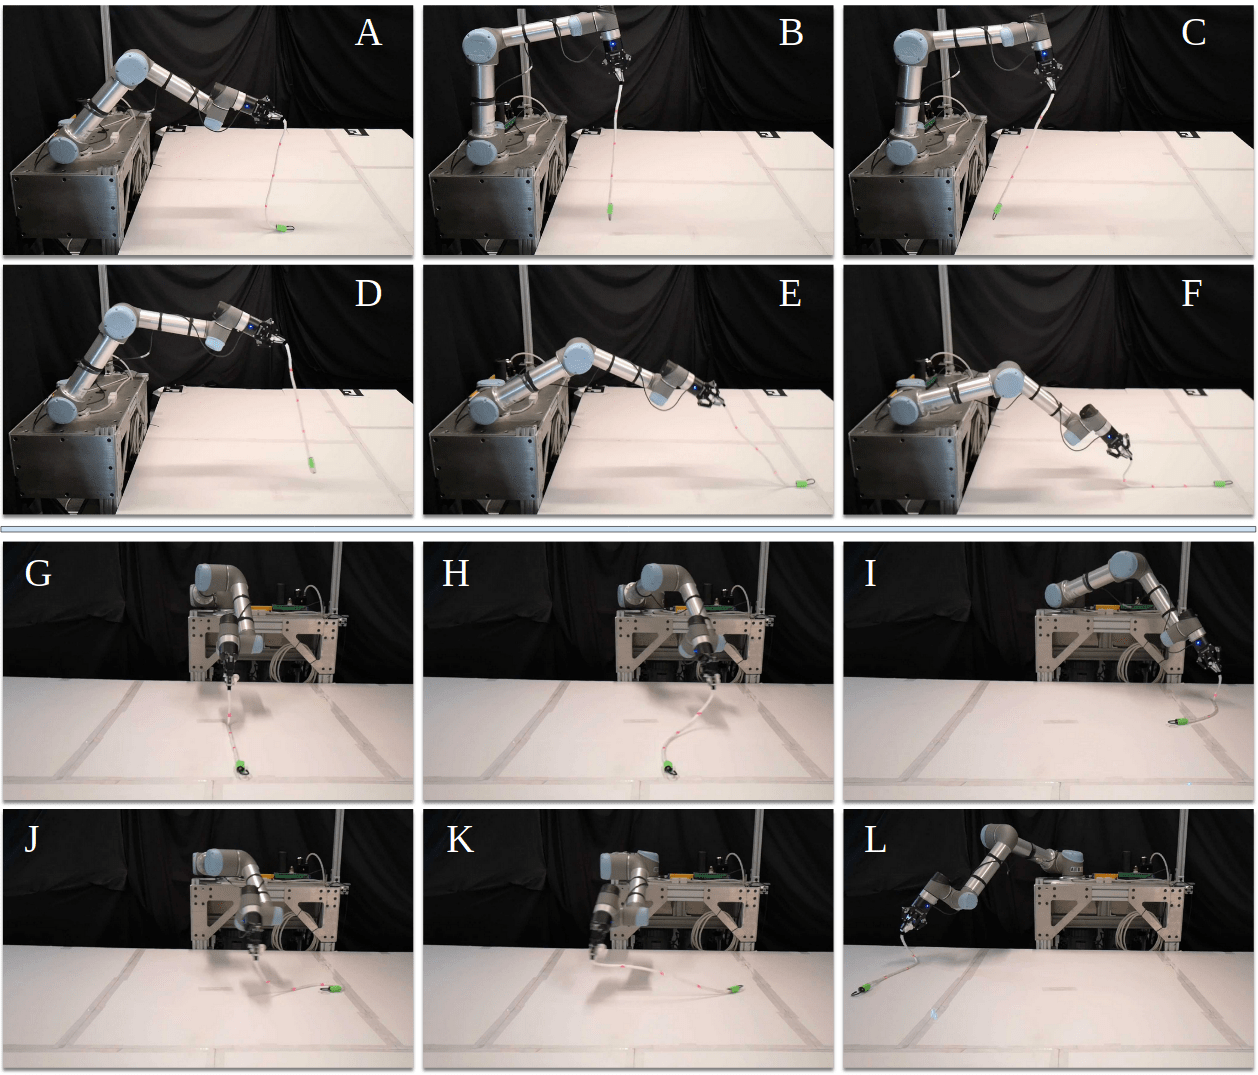
\includegraphics[width=0.49\textwidth]{teaser-v02-min.png}
\caption{
Overview of the proposed dynamic cable manipulation procedure with a UR5 robot. Each manipulation consists of a reset procedure (Section~\ref{sec:resets-repeat}) followed by a dynamic planar action (Section~\ref{ssec:action}) with two waypoints. The top two rows show a frame-by-frame side view of the UR5 as it resets by letting the cable settle (A,B), pulling back (C), casting forward (D,E), and dragging back slightly (F). After the reset, the bottom two rows show a frame-by-frame frontal view as the UR5 pulls towards one waypoint (G,H,I) and then towards the second waypoint (J,K,L) in an effort to get the cable endpoint to reach a desired target. \daniel{Draft figure. Should highlight cable (I think we can do in image editing software). Also wondering if side views and front views are OK. We could also overlay some arrows.}
}
\vspace*{-10pt}
\label{fig:teaser}
\end{figure}

The contributions of this paper are:
\begin{enumerate}
    \item Formulation of the dynamic planar manipulation of free-end cables.
    \item A simulation platform that accurately models dynamic planar cable manipulation.
    \item A dataset from 600 physical trials with 3 cables and the UR5 robot.
    \item Physical experiments with a UR5 robot and 3 cables \jeffi{suggesting that ...}.
\end{enumerate}
Supplementary material is available at 
\url{https://tinyurl.com/dyncable}.

%\begin{figure}[t]
%\center
%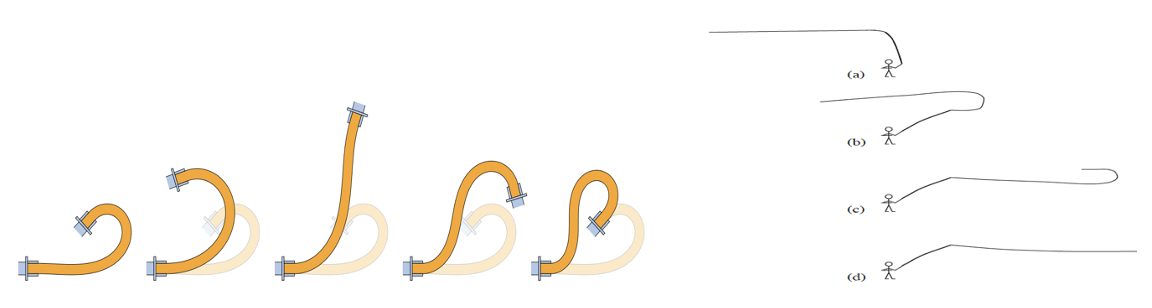
\includegraphics[width=0.49\textwidth]{overview.png}
%\caption{
%\Lawrence{Maybe we should illustrate the cable movement through time, divided into different stages as in the fly fishing papar? The figure on the left would look very nice but the fly fishing illustration may be also okay. We can potentially show the target, the two waypoints, robot actions, and the motion of the cable between stages as a sequence in one picture.} \daniel{I recommend removing this figure.}
%}
%\vspace*{-10pt}
%\label{fig:overview}
%\end{figure}




\section{Related Work}\label{sec:rw}

This paper builds on extensive prior research in data-driven robotics, deformable object manipulation, and dynamic manipulation. While using learned, data-driven techniques for robot manipulation has become a highly effective technique for generalizing to a wide variety of objects, as judged from strong empirical results~\cite{levine_finn_2016,mahler2019learning,dense_object_nets_2018,QT-Opt,openai-dactyl,rubik_cube_2019}, the majority of approaches focus primarily on manipulation of rigid objects in largely static settings such as a bin with objects, in contrast to the dynamic setting we consider with a deformable free-end cable.

\subsection{1D Deformable Object Manipulation}

Manipulation of 1D deformable objects such as cables has a long history in robotics research. Some representative applications include surgical suturing~\cite{robot_heart_surgery_2006,schulman_case_study_2013,suturing_autolab_2016}, knot-tying~\cite{van_den_berg_2010,case_study_knots_1991,knot_planning_2003,tying_precisely_2016}, untangling ropes~\cite{rope_untangling_2013,grannen2020untangling,tactile_cable_2020}, deforming wires~\cite{wire_insertion_1996,wire_insertion_1997}, and inserting cables into obstacles~\cite{tight_tolerance_insertion_2015}. We refer the reader to Sanchez~et~al.~\cite{manip_deformable_survey_2018} for a survey. % would be nice to say "a recent survey." but is 2018 considered "recent"? :) -JI

There has been a recent surge in using learning-based techniques for manipulating cables towards target configurations. A common setting is to employ pick-and-place actions with quasistatic dynamics, meaning that the robot slowly deforms the cable through a series of small adjustments, while allowing the cable to settle between actions. Under this paradigm, prior work has focused on cable manipulation strategies via techniques such as learning from demonstrations~\cite{zeng_transporters_2020,seita_bags_2021}, self-supervised learning~\cite{nair_rope_2017,ZSVI_2018}, generative modeling~\cite{wang_visual_planning_2019}, state estimation~\cite{state_estimation_LDO}, and dense object descriptors~\cite{priya_2020}. Prior work has also explored the use of simulators~\cite{mujoco,corl2020softgym} to train cable manipulation policies using reinforcement learning for eventual transfer to physical robots~\cite{lerrel_2020,yan_fabrics_latent_2020}. In this work, we develop a simulator for dynamic cable manipulation to accelerate data collection for training policies, with transfer to a physical UR5 robot.

Other cable manipulation settings that do not necessarily assume quasistatic dynamics include sliding cables~\cite{one_hand_knotting_tactile_2007,zhu_sliding_cables_2019} or using tactile feedback~\cite{tactile_cable_2020} to inform policies. This paper focuses on dynamic planar actions to manipulate cables from one configuration to another.


\subsection{Dynamic Manipulation of Cables}

In dynamic manipulation settings, a robot takes actions rapidly to quickly move objects towards desired configurations, as exemplified by applications such as swinging items~\cite{swingbot_2020,diabolo_2020} or tossing objects to target bins~\cite{zeng_tossing_2019}. As with robot manipulation, these approaches tend to focus on dynamic manipulation of rigid objects.

A number of analytic physics models have been developed to describe the dynamics of moving cables, which can then be used for subsequent planning. For example, Gatti-Bono and Perkins~\cite{fly_fishing_2004} present a two-dimensional dynamic casting model of fly fishing. They model the fly line as a long elastica and the fly rod as a flexible Euler-Bernoulli beam, and propose a system of differential equations to predict the movement of the fly line in space and time. 
In contrast to continuum models, Wang and Wereley~\cite{wang2011analysis} propose using a finite-element model to represent the fly line by a series of rigid cylinders that are connected by massless hinges. These works focus on developing mathematical models for cables, and do not test on physical robots.
%While finite element models are widely used in motion planning for deformable objects manipulation~\cite{yoshida2015simulation,duenser2018interactive,li2018model}, these works tend to focus on tasks where quasistatic assumptions may be tasks assumpdifferent tasks such as .
%See~\cite{li2018model} for a review on model-based manipulation planning of deformable objects.

In the context of robotic dynamic-cable manipulation,
Yamakawa~et~al.~\cite{dynamic_knotting_2010,yamakawa2012simple,high_speed_knotting_2013,one_hand_knotting_tactile_2007} demonstrate that a high-speed manipulator can effectively tie knots by initially whipping cables upwards. Since their robot arms move at high speeds, they are able to simplify the modelling of cable deformation by assuming each cable component follows the robot end-effector motion with constant time-delay. Kim and Shell~\cite{kim2016using} study a novel robot system with a flexible rope-like structure attached as a tail that can be used to strike objects of interest at high speed. This high-speed setting allows them to construct primitive motions that exploit the dynamics of the tail. They adopt the Rapidly-exploring Random Tree (RRT)~\cite{RRT_2001} and a particle-based representation to address the uncertainty of the object’s state transition. In contrast to these works, we aim to control cables for tasks in which we may be unable to rely on these simplifying assumptions.

%In the context of cable manipulation, Yamakawa~et~al.~\cite{dynamic_knotting_2010,yamakawa2012simple,high_speed_knotting_2013,one_hand_knotting_tactile_2007} focus on dynamic manipulation of cables using robot arms moving at high speeds, enabling them to model cable deformation algebraically under the assumption that the effect of gravity is negligible. \raven{yeah, I think we also assume the gravity is negligible but should we point this out here?} Results show that a single multi-fingered robot arm can effectively tie knots by initially whipping cables upwards. As we are interested in getting cable endpoints to reach desired targets that may be far from the robot end effector's range of motion, it is infeasible to assume a model where each cable component follows the robot end-effector motion with constant time-delay, as in Yamakawa~et~al. Instead, we use a learning-based method.

%Kim and Shell~\cite{kim2016using} use a small-scale mobile robot with a cable attached as a tail to manipulate small objects by leveraging inter-object friction to drag or strike the object of interest. While their work aims to tackle dynamic cable control, it relies heavily on physics models for motion primitives that are only applicable to dragging objects via cables, and uses a RRT-based graph search algorithm to address the stochasticity in the system. \daniel{Will revise (Prof G 3/1 feedback)} We avoid the modeling of the cable physics and we aim to control cables for tasks which dynamically cannot rely on the same dragging motion primitives.

%Drigalski~et~al~\cite{diabolo_2020} present an approach for robots to play diabolo \raven{should we not cite this paper or make this citation more related to our study?}. They train agents manipulating two sticks connected by a string, and the model is run on a dual robot arm system. The arms perform dynamic, swinging motions on the gripped sticks and string to manipulate the diabolo. In their work, they use an analytical model to predict the diabolo’s motion as a function of the sticks’ trajectory. \daniel{Will revise (Prof G 3/1 feedback)} In this paper, we use a learned model to predict the cable endpoint position given an action and we are interested in finding the action to produce a certain cable configuration.

%\Lawrence{I am summarizing this very new paper Adi brought up. I think that is more related to our setting than Harry's paper since it is also doing free-end.}

Two closely related prior works are Zhang~et~al.~\cite{harry_rope_2021} and Zimmermann~et~al.~\cite{zimmermanndynamic}. Zhang~et~al.~\cite{harry_rope_2021} propose a self-supervised learning technique for dynamic manipulation of fixed-end cables for vaulting, knocking, and weaving tasks. They parameterize actions by computing a motion using a quadratic program and learning the apex point of the trajectory. In contrast to Zhang~et~al., we use \emph{free-end} cables. Zimmermann~et~al.~\cite{zimmermanndynamic} also study the dynamic manipulation of deformable objects in the free-end setting. They model elastic objects using the finite-element method~\cite{bathe2006finite} and use optimal control techniques
%including Newton's method and Differential Dynamic Programming
to solve trajectory optimization problems. They study the task of whipping, which aims to find a trajectory such that the free end of the cable hits a predefined target with maximum speed, and laying a cloth on the table. Their simulated motions perform well for simple dynamical systems such as a pendulum, but since their model depends on good parameter estimation, its performance decreases for more complex systems like soft bodies due to mismatch between the simulation and the real world. In contrast, we adopt a learned, data-driven technique for robotic manipulation of free-end cables, focus on planar manipulation, and are interested in finding the best action such that the free end of the cable achieves a target position on the plane.

\section{Problem Statement}\label{sec:PS}

We consider a 6-DOF robot arm which controls a free-end cable and continually grips one end of the cable throughout each dynamic motion. We assume a planar setup where the cable endpoint lies on the plane and the robot end-effector takes actions at a fixed height slightly above the plane. The full configuration of the cable and the environment is infinite dimensional and complex to model, and we are interested in the cable endpoint. Thus, we concisely represent the state as ${\state=(r, \theta)}$, indicating the endpoint position on the plane in polar coordinates, and where the robot base is located at $(0, 0)$. The objective is to train a parameterized inverse model $f_{\rm inv}$ which, when given the desired target ${\state^{(d)}=(r_d, \theta_d)}$ for the cable endpoint, produces a one-step arm motion ${\ba=f_{\rm inv}(\state^{(d)})}$ that robustly achieves $\state^{(d)}$. We assume access to a dataset of $N$ pairs of end positions and actions, denoted as ${\mathcal{D} = \{ (\state^{(d)}, \ba)^{(i)} \}_{i=1}^N}$ to supervise $f_{\rm inv}$.


\jeffi{I think we need to provide an overview of the method, including resets/repeatability, sim-to-real, and the rest, before jumping into resets and repeatability.  I also recommend we top-level sections that are abstract, e.g. "Preliminaries", "Background", "Setup", "Method", etc...  So "Resets and Repeatability" and "Simulation to Reality" would be either under their own top-level section, or moved into the Methods section.}
\Vincent{Perhaps saying we train $f_{\rm inv}$ is a little confusing when later we train a forward dynamics model and sample from that?}
\section{Resets and Repeatability}\label{sec:resets-repeat}

The first step in dynamic cable manipulation is to determine a highly repeatable \emph{reset state}, a position that the cable can be quickly and reliably manipulated into. We propose the following reset procedure \jeffi{we may consider defining a general reset procedure/method, and leave the specific one below to the experiments section.  The idea being to keep the method description here high-level, and use the experiments as an ``instantiation'' of the method.}:

\begin{enumerate}
\item Lift the cable vertically up with the free endpoint touching the work surface to prevent the cable from dangling.
\item Continue to lift the cable up such that the free endpoint loses contact with the surface.
\item Let the cable hang for 3 seconds to stabilize. \raven{I changed the reset motion as you suggested. However, we still need to hang up for a few sec since there could be some dangling after we lift it up. At the very beginning, without step 1 and 2, we have to wait for 20 seconds. Now we just need to wait 3s to entirely stabilize the cable.}
\item Perform a motion to swing the free endpoint forward to land on the surface, then slowly pull the cable towards the robot until the reset position is reached.
\end{enumerate}

We execute this reset motion before each dynamic planar cable manipulation action to ensure the same initial cable configuration. Figure~\ref{fig:teaser} (top half) shows a frame-by-frame overview of the reset procedure. After this reset procedure, we assume that the robot end-effector performs dynamic manipulation at a fixed height.

\section{Simulation to Reality}\label{sec:simulator}

\begin{figure}[t]
\center
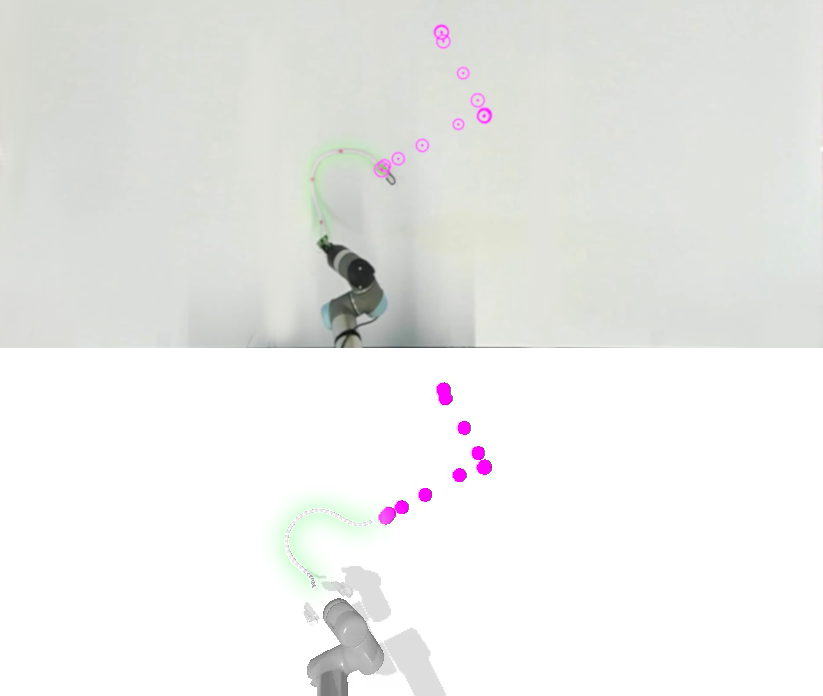
\includegraphics[width=0.49\textwidth]{sim_real.png}
\caption{
\textbf{Above:} The extracted cable endpoint positions at each time step spaced 100 milliseconds apart. The pixel coordinates of each waypoint are converted to simulation coordinates using x reference points.
\textbf{Below:} The same trajectory is run in the simulator, and the distance between the cable endpoint and the waypoint at each time step is used as a metric to for optimizing the simulation parameters. In this example, the simulated endpoint location matches the ground truth endpoint location, but the cable configuration is different, demonstrating a limitation with the optimization metric. The cables are highlighted for the purpose of visibility.
}
%\vspace*{-10pt}
\label{fig:tasks-1}
\end{figure}
  
We create a simulation environment to efficiently collect data for policy training. In PyBullet~\cite{coumans2019} simulation, cables consist of capsule-shaped rigid bodies held together by 6-DOF spring constraints. We denote the collective set of PyBullet simulation parameters as $\theta_{\rm sim}$. For each trajectory $m_j$ in the training set of $M$ total \emph{physical} trajectories, we record the 2D location of the cable endpoint, $p_t = (x_t, y_t)$ \jonathan{Earlier we refer to endpoints in polar coordinates, we need to keep it consistent}, at each time step $t$ spaced \SI{100}{\milli\second} apart \jonathan{Consider moving this section \ref{sec:simulator} after section \ref{ssec:action}, where we can define planar actions and corresponding trajectories}. The tuning objective is to find parameters $\theta_{\rm sim}$ that minimize the average $L^2$ distance between the cable endpoint in simulation, $\hat{p}_t = (\hat{x}_t, \hat{y}_t)$, to the real waypoint at each $t$:
\begin{equation}\label{eq:tuning}
    \minimize_{\theta_{\rm sim}} \;\; \epsilon_{\rm trajs} = {\sum_{j}^M{\sum_i^{N_j}{\lVert p_i - \hat{p}_i \rVert}_2}}.
\end{equation}
The number of waypoints compared for each trajectory is $N_j = \lfloor {T_j}/{100} \rfloor$, where $T_j$ is the duration of $m_j$ in milliseconds. For each cable, we collect 60 physical trajectories and evaluate on an additional 20 trajectories where $(\theta_1, \theta_2, r_2, \psi)$, for each trajectory are uniformly sampled. Increasing the number of trajectories to 80 led to an increase in the validation metric $D$ by $2\% - 12\%$, suggesting that additional trajectories would not improve tuning. \daniel{Above text needs work, we're using notation before we define it, and we are talking about physical trajectories (not resets!) before we define what those are.} \jeffi{Also... we should keep this at a higher level, and move the 60 vs 80 discussion to experiments and discuss as part of ablations or similar discussion.}


\subsection{PyBullet Simulation Parameter Tuning}

% \daniel{While this section is improved since last draft as per Prof G feedback, I recommend moving details of DE to the Appendix. (Edit: done?)} 

To tune parameters more efficiently compared to grid search or random search~\cite{random_search_2012}, we search for parameters using Differential Evolution (DE)~\cite{de_tuning_2020}. We do this because DE does not require a differentiable optimization metric, and is more efficient than grid search and Bayesian optimization, which both scale poorly with a large number of parameters. Grid search runtime is exponential in the number of parameters, while evolutionary algorithms allow for a variable stopping condition. \jeffi{Is the previous statement backed up by Collins~et~al.~\cite{de_tuning_2020}?  If so, we should state that clearly.  Otherwise this statement needs more justification.} At generation $0$, the algorithm initializes a size $N$ population of candidate parameter vectors via Latin Hypercube sampling. After each generation, each parameter vector in the current generation produces a `child' vector, which each element in the vector is derived from a combination of the parent, the best-performing individual in the current generation, and $2$ random population members. This heuristic permits enough stochasticity to sufficiently explore the parameter search space, while converging toward an optimum.

Table~\ref{tab:hparams-sim} \jonathan{This table is now in the Appendix} lists the simulation parameters we tuned, which we chose based on intuition of the parameters that best capture cable physics. Comparing the selected parameters with Collins~et~al.~\cite{de_tuning_2020}, who explore a similar physics engine tuning problem, we also optimize over mass, lateral friction, rolling friction, sliding friction, linear damping, and angular damping. Two other parameters the authors claim were most influential were time step and maximum joint velocity. We do not vary PyBullet's time step because decreasing it from 1/480s causes the cable, modeled as discrete capsules, to exhibit unstable behavior such as breaking apart, while increasing the time step greatly decreases the simulation speed. We find that running DE with the maximum joint velocities as parameters as opposed to the original set increased the deviation in cable trajectory by 11\% for one cable, most likely due to an increase in the search space. Tuning maximum joint velocities also increases the duration of the algorithm by 60\% due to an additional 6 parameters to the population size.

Table \ref{tab:tuning} compares similarity between cable behavior in simulation and reality. For each cable, DE was able to reduce the discrepancy in the cable endpoint location throughout and after the trajectory, compared to PyBullet's default parameter settings. Despite the tuning, results suggest a reality gap in cable behavior still remains, motivating the use of the fine-tuning procedure discussed in Section~\ref{ssec:supervised}.

% Daniel: let's keep tables at the top of the page using [t].
\begin{table}[t]
  \setlength\tabcolsep{5.0pt}
  %\vspace{-1em}
  \centering
  \caption{
    Results for the differential evolution algorithm on a set of 20 validation trajectories over all 3 cables (see Figure~\ref{fig:cables}). The two metrics considered are final $L^2$-distance, which is the 2D Euclidean distance between endpoint locations between simulation and reality after a trajectory terminates, and $\epsilon_{\rm trajs}$, defined in Equation $\ref{eq:tuning}$. We compare the performance of parameters found by DE with that of PyBullet's default parameter settings. Values are averaged across the 20 trajectories, and expressed in percentages of cable length.
  }
  \small
  \begin{tabular}{@{}lllll}
  \toprule
  Metric & Cable 1  & Cable 2  & Cable 3  \\
  \midrule
  (Default) Final $L^2$-distance & 38.2\% & 27.5\% & 27.5\% \\
  (Default) $\epsilon_{\rm trajs}$ & 38.2\% & 29.4\% & 24.5\% \\
  (DE) Final $L^2$-distance & \textbf{20.5}\%  & \textbf{19.2}\% & \textbf{16.6}\% \\
  (DE) $\epsilon_{\rm trajs}$ & \textbf{28.4}\% & \textbf{23.4}\% & \textbf{18.7}\% \\
  \toprule
  \end{tabular}
  %\vspace{-0.5em}
  \label{tab:tuning}
\end{table}  


\section{Method}\label{sec:method}

In this section, we describe how we propose to address dynamic manipulation of free-end cables, including the action parameterization and the supervised learning procedure. We use this procedure to deploy 2D planar manipulation on a physical UR5 robot.

\subsection{Planar Action Parameters}\label{ssec:action}

Each action $\ba$ defines a dynamic trajectory of the robot.

% For the 2D planar manipulation task, we define and test with two action parameterizations. The first action is parameterized by five scalar quantities:
% \begin{equation}\label{eq:act1}
%     \ba = (x_1, y_1, x_2, y_2, v_{\rm max})
% \end{equation}
% which represents two points in the plane (which assumes a fixed height), and $v_{\rm max}$ represents the maximum velocity allowed for the robot. 

\daniel{I think we need better justification for the action params -- section is major WIP, will work on it.} We define and test with the action parameterizations that replicate recorded human-generated trajectories of free driving the robot to dynamically move the cable towards a target. We notice the trajectories can be represented by two splines that are parameterized in polar coordinates. We choose to use two splines as opposed to one because the second spline is required to produce an inertial planar motion that accelerates the endpoint in the direction of the end effector's velocity. \jonathan{Possibly support the reasoning with the coverage metric of using a single spline} \jonathan{Need to revise the reasoning and better integrate it with below explanation} \daniel{easy workaround: do with 1 spline, show it is bad}

We represent the robot as a 3 joint mechanism in the global frame: a rotation joint at the base $\phi_1$, a prismatic joint $d_2$ along the direction from the base to the wrist, and a rotation angle $\phi_3$ with respect to $d_2$. In the polar coordinate frame, we define $(r, \theta)$ to be the position of the end effector, and $\psi$ as the angle of the wrist. Using a standard IK solver, the 6-DOF robot can achieve any $(\phi_1, d_2, \phi_3)$, which corresponds to moving the end effector to $(r, \theta, \psi)$ in polar space.


Each action is parameterized by a fixed set and a variable set of parameters, which we refer to as \emph{system parameters} and \emph{action parameters}, respectively. The system parameters are $r_0$, the 2D distance from the reset position of the end effector to the origin in the polar coordinate frame, and $\vmax$, the linear velocity of the end effector. The $r_0$ can be modified to produce trajectories that vary in curvature, as seen in Figure~\ref{fig:spline}. Larger values for $r_0$ will produce ``flatter'' splines whereas smaller values will produce splines with more curvature. In practice, we find that the flatness of the action and the maximum velocity $\vmax$ in the jerk-limited motion significantly impact the cable endpoint coverage over the workspace. \daniel{Need plots / results!} To find the best $(r_0, \vmax)$ that generate actions with maximum coverage, we perform grid search in the PyBullet simulator and choose the combination with maximum coverage as in Section~\ref{sec:experiments} \daniel{Section reference does not make sense here}. Once we select the system parameters, they are fixed and not included in the actions $\ba$ for learning the inverse model $f_{\rm inv}$.

We consider two sets of action parameters. The first consists of three values:
\begin{equation}\label{eq:act2}
    \ba = (\theta_1, \theta_2, r_2).
\end{equation}
With a fixed reset location $(r_0, \theta_0)$ given by the reset motion in Section~\ref{sec:resets-repeat}, the trajectory of the end effector passes through two waypoints $(r_1, \theta_1)$ and $(r_2, \theta_2)$ in polar space while maintaining a fixed height, as shown in Figure~\ref{fig:spline}, where $\theta$ changes with jerk-limited, maximum velocity $\vmax$. A limited jerk velocity reduces the stochasticity brought by a jerk-intensive motion. The $r$ changes from $r_0$ to $r_2$ using a cubic spline $f(t)$ as a function of time, where $f'(t_{r_0}) = f''(t_{r_0}) = f'(t_{r_2}) = f''(t_{r_2}) = 0$. \jonathan{TODO Verify this is accurate}. Here, $r_1$ is equal to $f(T_{\theta_1})$, where $T_{\theta_1}$ is the time it takes to change from $\theta_0$ to $\theta_1$. \raven{Jeff would be the best person to further explain this.}
% $\theta_1$ and $\theta_2$ translate to rotation of the base joint, while $r_2$ translates to rotation in the shoulder and elbow joints. By keeping most of the joints besides the base joint fixed throughout the trajectory, we reduce unnecessary motions that contribute to unpredictable cable behavior.
% Because we deal with 2D planar manipulation, the $z$ coordinate is fixed throughout the trajectory.

\raven{This is hard to explain and we need to discuss how to make this clear. Basically, when we generate the spline action, we didn't generate in the polar coordinate whose origin is the robot base. Since we just want to generate the spline action with the starting point ($r_0$, $\theta_0$) fixed, we can do this in the action space. Since $r_0$ is directly related to the flatness of the generated spline, if we want to generate actions with different flatness, we need to change $r_0$. However, the reset position is fixed in real and we can only move the origin further or near to change $r_0$. I hope this could explain this better but again Jeff would be the best person to explain. }

% The polar coordinate parameters are in a different coordinate space than the real world coordinate space. For instance, the fixed parameter $r_0$ does not represent the physical distance between the robot base and the end effector. 

We notice the coverage space for actions with the above three parameters is limited in practice (see Figure \ref{fig:coverage}). Taking inspiration from human generated action \daniel{this is not scientific} and verifying our intuition with physical motions (Section \ref{ssection:protocol}), we include a fourth parameter, the wrist rotation angle $\psi$ around the z-axis, resulting in:
\begin{equation}\label{eq:act2_wrist}
    \ba = (\theta_1, \theta_2, r_2, \psi).
\end{equation}
During the trajectory, the end effector follows the spline parameterized by $(\theta_1, \theta_2, r_2)$, and for the portion of the trajectory from $(r_1, \theta_1)$ to $(r_2, \theta_2)$, the wrist rotates $\psi - \theta_2$ radians with a maximum velocity, jerk-limited rotation. In an ablation study in \daniel{insert section}, we examine the impact of the wrist angle parameter.

% For both splines, 
% the maximum change in radians per second of the angle of the end effector $\theta$ is set to 2 radians/s, which is fast enough to produce a large range of reachable cable endpoints, but not so fast such that the cable is uncontrollable. 
% the maximum acceleration and jerk are set at maximum values according to the UR5 specification. A standard IK solver is applied to convert the end effector trajectory from coordinate space into joint space.

\begin{figure}[t]
\center
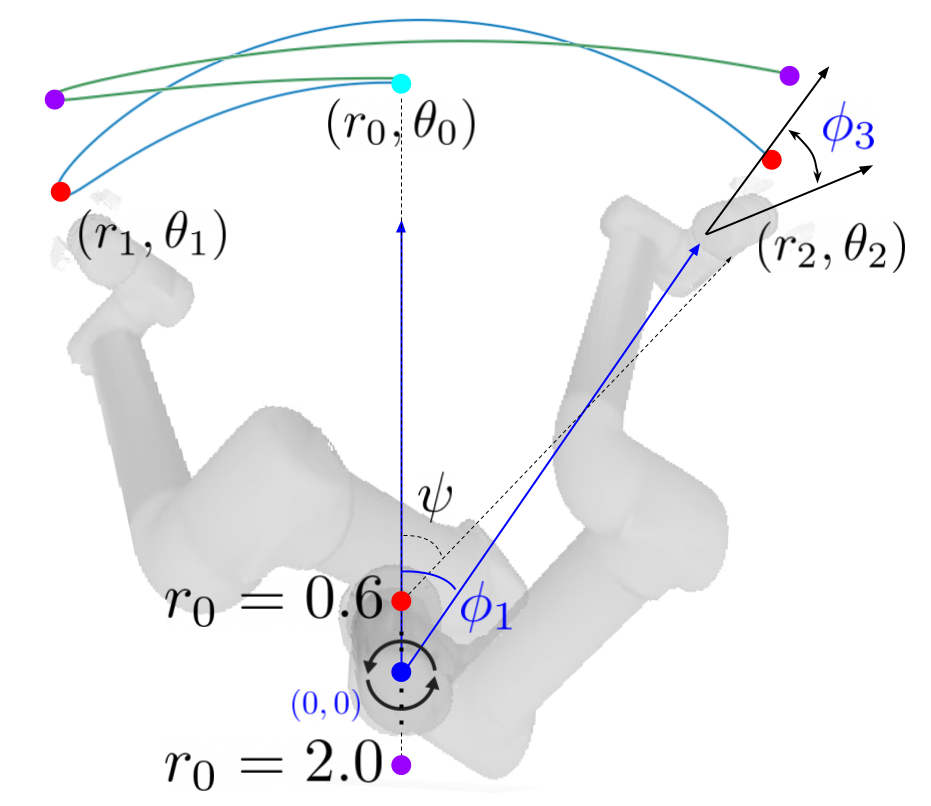
\includegraphics[width=0.49\textwidth]{spline_figure.png}
\caption{
Example of two sets of splines that are traced by the end effector during the trajectory (Equation \ref{eq:act2}) (not drawn to scale) of the UR5, for two different $r_0$ values: $r_0 \in \{0.6, 2.0\}$. The reset procedure brings the end effector to $(r_0, \theta_0)$ in the polar space before the start of each dynamic motion. Decreasing $r_0$ increases the curvature of the trajectory. \daniel{draft figure, but much improved! We need to make wrist rotation clear, and adjust as per Prof Goldberg's feedback (e.g., showing consistent coordinate systems) Also, we show $\phi_1$ and $\phi_3$ but not $d_2$, and the $\psi$ could be visualized better maybe with an inset image? Finally use $r_0=2.0$ instead of just 2.}
}
%\vspace*{-10pt}
\label{fig:spline}
\end{figure}


\subsection{Supervised Learning Procedure}\label{ssec:supervised}

% Daniel: describe how we made the figure here (makes it easier later when we have to reproduce or change things).
% Repeatability analysis code: https://drive.google.com/drive/u/1/folders/1lOLcdcte6Y93qHPSpJW4S0B8wxWaAS4O
% Cable coverage code: https://drive.google.com/drive/u/1/folders/1mue6nc8kTV23KwfAd06cI6mjy87W531B
% \begin{figure}[t]
% \center
% 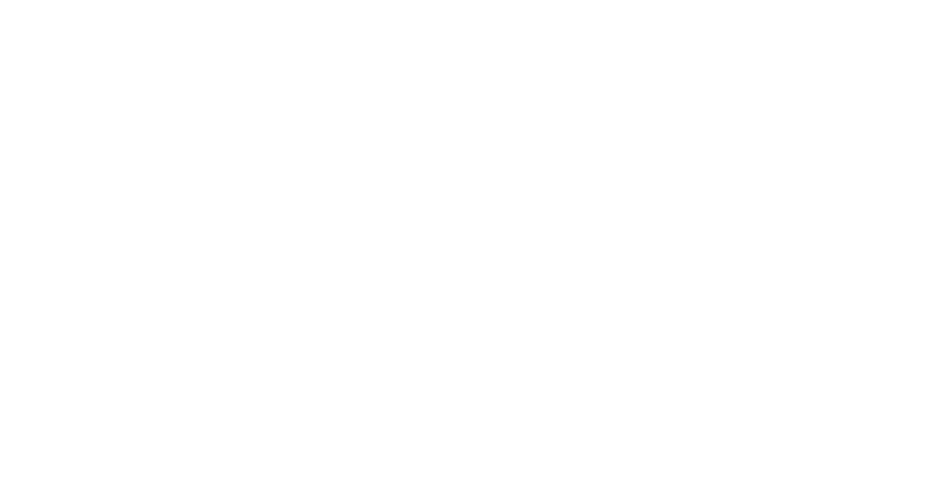
\includegraphics[width=0.49\textwidth]{empty.png}
% \caption{
% \daniel{TODO show the figure Jonathan has where he samples the grid, has the robot aim to cast the cable endpoint out to the end, then pulls back ...}
% }
% %\vspace*{-10pt}
% \label{fig:sampling-1}
% \end{figure}

The inverse model $f_{\rm inv}$ consists of sampling multiple input actions $\ba$, passing each action through a forward dynamics model $f_{\rm forw}$ that outputs the predicted cable endpoint location $(\hat{x}, \hat{y})$, and selecting the optimal $\ba$. We use a feedforward neural network for this forward dynamics model, with 4 fully connected layers with 256 hidden units each.  \daniel{Now we're talking Cartesian coordinates, whereas earlier it seems like everything was in polar coordinates. We should find a way to make all this clear.} 

We first generate dataset $\mathcal{D}_{\rm real}$ for each cable using real trajectories, by grid sampling $\theta_1$, $\theta_2$, $r_2$ and $\psi$. Collecting data for 200 trajectories takes approximately one hour, motivating the need for more efficient data generation in simulation.

\raven{will revise according to Prof.G's note 0301}To facilitate data-efficient training in simulation, we take inspiration from Hindsight Experience Replay (HER)~\cite{HER_2017} by executing an action and pretending a target was at the final endpoint location. For generating training data $\mathcal{D}_{\rm sim}$ in PyBullet simulation, we sample each parameter $\theta_1$, $\theta_2$, $r_2$, and $\psi$ independently from a uniform distribution. The uniform distribution bounds for $\theta_1$, $\theta_2$, $r_2$ and $\psi$ are set to be as wide as possible such that the end effector stays within a reachable, collision-free bounding area during the trajectory. We then execute the action in a simulator tuned using real data as discussed in Section \ref{sec:simulator}, record the corresponding cable endpoint location after the action terminates and store it as a transition $(\ba, \bs)$. We generate 36,000 such transitions and train $f_{\rm forw}$ to predict $\bs$ given $\ba$ on the simulated transitions. \daniel{please formalize this network with math notation somewhere, also people who don't know HER will likely not understand.} We transfer the trained dynamics model to real by executing 200 grid-sampled actions again in the physical setup, recording the transitions and fine-tuning the dynamics model using those transitions.

Taking advantage of the symmetrical aspect of the problem, actions in all datasets are sampled such that $\theta_1 < 0$, $\theta_2 > 0$, and $\psi > 0$, to obtain targets on the right of the workspace axis of symmetry. If $(\theta_1, \theta_2, r_2, \psi)$ produces target $(r_d, \theta_d)$, $(-\theta_1, -\theta_2, r_2, -\psi)$ will produce $(r_d, -\theta_d)$. Therefore, during evaluation, for targets $(r_d, \theta_d)$ on the left of the axis, we take $f_{\rm inv}(r_d, -\theta_d) = (\hat{\theta}_1, \hat{\theta}_2, \hat{r}_2, \hat{\psi})$ and output $(-\hat{\theta}_1, -\hat{\theta}_2, \hat{r}_2, -\hat{\psi})$.

% To mitigate distributional shift, we filter the dataset such that the targets are uniformly spread throughout the plane, by dividing the plane into equal-sized boxes and limiting the number of samples per box.


\section{Experiments}\label{sec:experiments}

In this section, we describe the experiments we perform in PyBullet simulation and on a physical UR5 robot.

\subsection{Baseline Methods}\label{ssection:methods}
% \jeffi{Do we mean \emph{Baseline Methods}?}

We benchmark performance of the forward dynamics model trained on (1) $\mathcal{D}_{\rm real}$ only, (2), $\mathcal{D}_{\rm sim}$ only, and (3)  $\mathcal{D}_{\rm sim}$ first, then fine-tuned on $\mathcal{D}_{\rm real}$. Along with these three forward models, we test with two baseline methods, one analytic and one learned:

\textbf{Polar Casting.} Given a target cable endpoint location $(r_d, \theta_d)$, first perform a casting motion that causes the free endpoint to land at $(r_{\rm max} + r_c, \theta)$, where $r_{\rm max}$ is the maximal distance from the base to the robot wrist, and $r_c$ is the cable length. To perform this motion, the robot rotates $\theta_d$ radians, and executes a predefined casting motion. After the casting motion, the robot slowly pulls the cable toward the base for a distance of $r_{\rm max} + r_c - r_d$. Targets $(r_d, \theta_d)$ achievable by this method are limited to the circular segment seen in figure \ref{fig:coverage}. In Cartesian coordinates, the arm is limited to a minimum $y$ coordinate of $\SI{0.466}{\meter}+r_c$ to prevent the end effector from hitting the robot's supporting table, where $\SI{0.466}{\meter}$ is the distance from the center of the robot base to the edge of the table. 

% $r_c \leq r_d \leq 1+r_c$, where $r_c$ is the cable length, as the robot cannot pull closer than $r_c$ without hitting the base. 
\Lawrence{I think this polar casting should be mentioned way earlier in the paper as a motivation for our method, and here bring it up again to remind the readers that our method indeed verifies our hypothesis that our method address the limitation of naive casting. We need motivation for why we choose these as baselines.} \daniel{Yes, show coverage. Also agree with Lawrence's comment here} 

\textbf{Forward Dynamics Model learned with Gaussian Process.}
While polar casting serves as an analytic baseline, we choose a Gaussian process model as a learning baseline to compare with the proposed deep neural network model. Gaussian process is a commonly used model in motion planning and machine learning~\cite{Gaussian_process_ML}. We train a Gaussian process regressor to predict the cable endpoint location  $(\hat{x}, \hat{y})$ given input action $\ba$ using the previously generated 36,000 transitions training data.

% \textbf{Actions with Polar Trajectory}. We plan through the learned dynamics model to output an action $\mathbf{a}$ that the robot executes by having the end effector follow the trajectory defined by the action parameterization. 
% \textbf{Actions without wrist rotation, $r_0 = 2$.} The forward dynamics model uses $(\theta_1, \theta_2, r_2)$ for each input action.
% \textbf{Actions without wrist rotation, $r_0 = 0.6$.}
% \textbf{Actions with wrist rotation, $r_0 = 0.6$.} The forward dynamics model uses $(\theta_1, \theta_2, r_2, \theta_{wrist})$ for each input action.

\subsection{Physical Setup}

We use a UR5 robot with three cables of different stiffnesses and diameters (Figure~\ref{fig:cables}). Each cable has a weighted attachment (a hook or a magnet \Lawrence{see overleaf comment, are we using it as a magnet?}) to resemble a home or industrial setting in which the passing of the cable sets up a downstream task such as plugging into a mating part. \daniel{Do we have a citation? I think this justification needs improving.}  \jeffi{I reworded to be less specific, do you think it needs a citation now?}

\begin{figure}[t]
  \center
  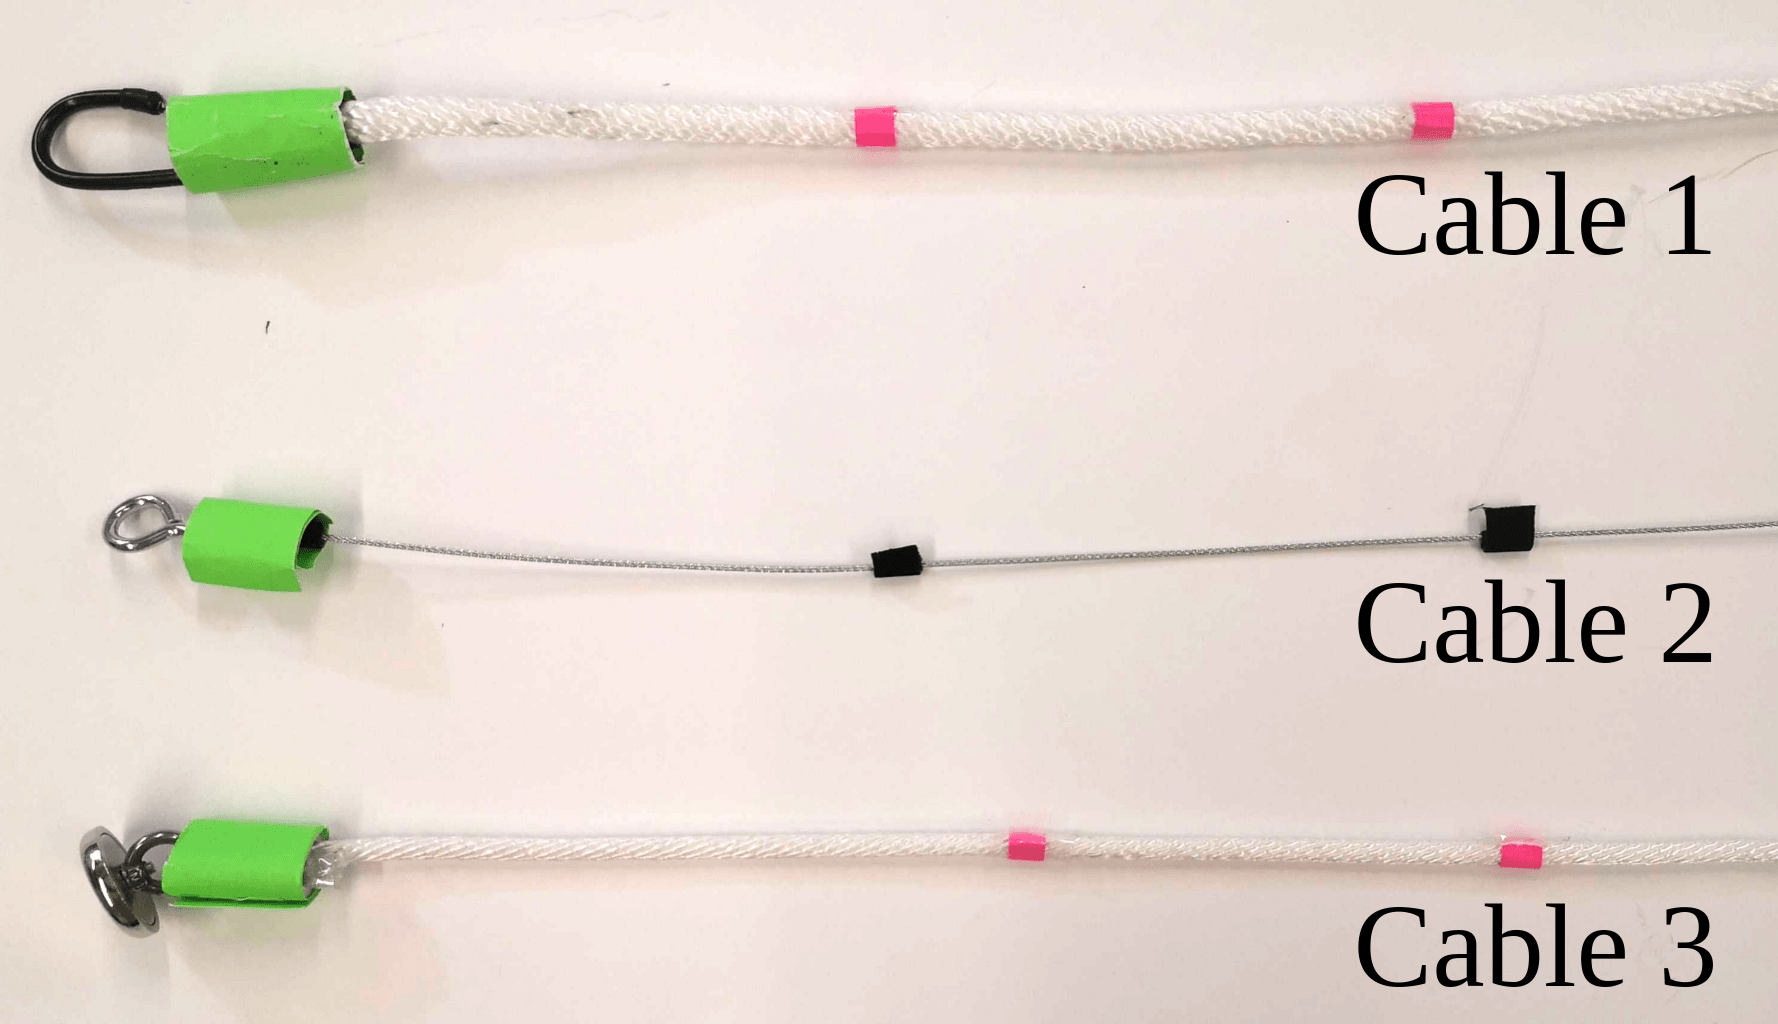
\includegraphics[width=\columnwidth]{figures/cables-brightened-v01-min.png}
  \caption{
  Three cables used in physical experiments, consisting of two polyester ropes and one braided iron wire. A mass is attached to each cable endpoint. From top to bottom, the cable lengths are \SI{0.62}{m}, \SI{0.65}{m}, and \SI{0.67}{m} without the attachment, and \SI{0.67}{m}, \SI{0.68}{m}, and \SI{0.68}{m} with the attachment. The cable diameters are \SI{11}{mm}, \SI{1.5}{mm}, and \SI{7}{mm}.
  }
  \label{fig:cables}
 % \centering
 % \begin{minipage}[b]{0.4\textwidth}
 %    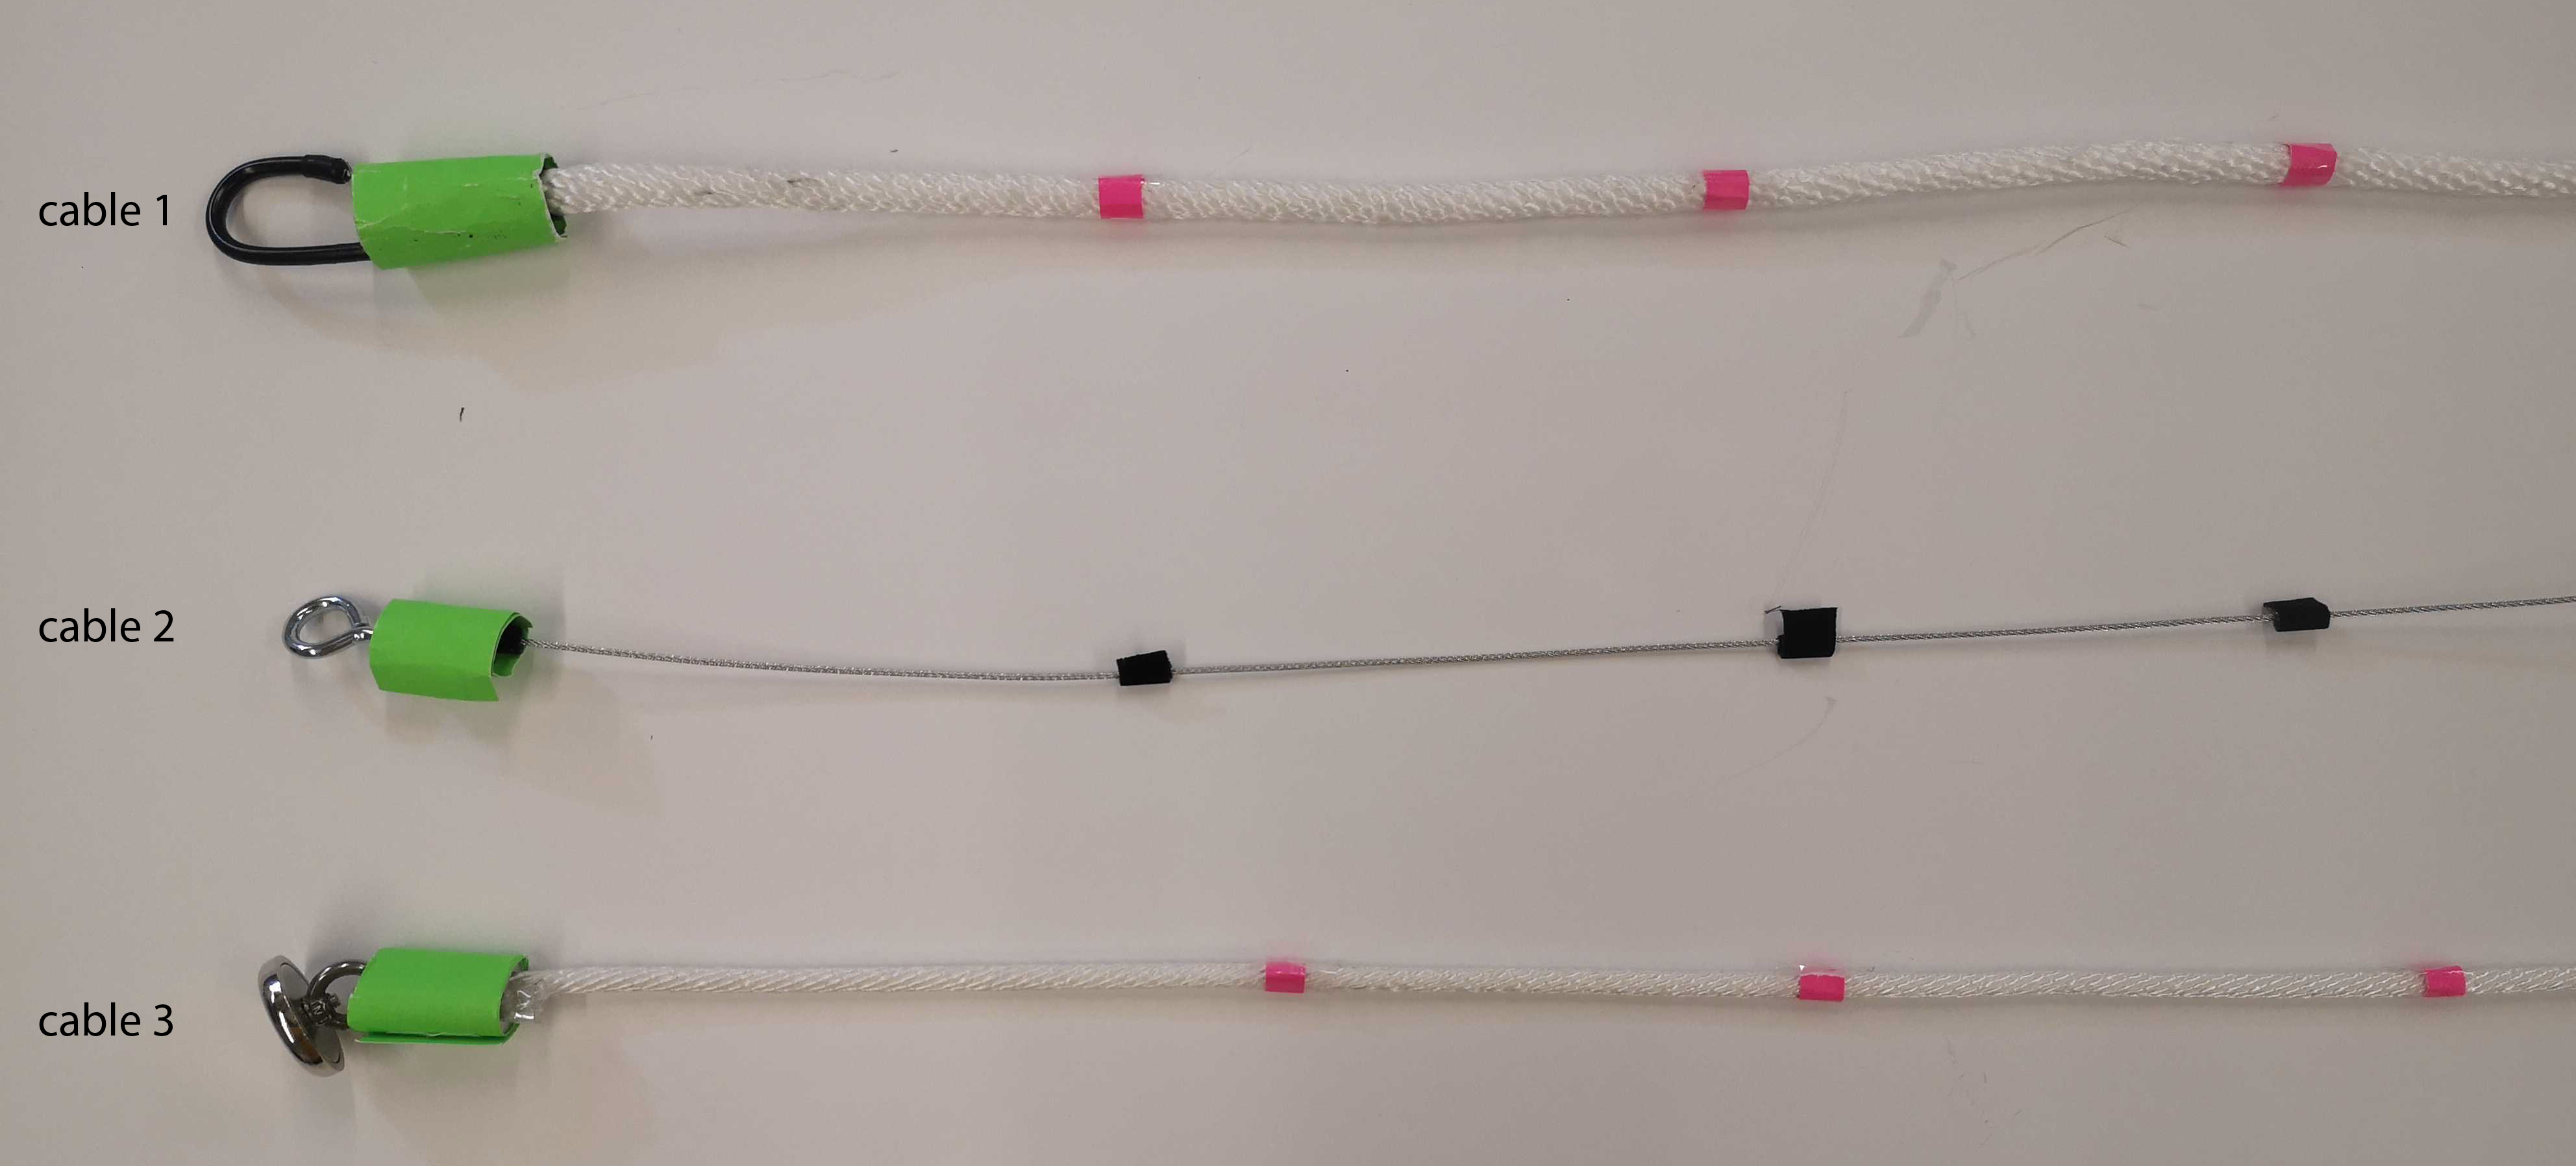
\includegraphics[width=\columnwidth]{figures/cables.png}
 %   \caption{
 %   Three cables used in physical experiments, consisting of two ropes and one braided wire. \daniel{make the text larger, describe the hooks, etc! (Edit: please make this figure wider and standalone, why is it combined with the below figure?)}
 %   }
 %   \label{fig:cables}
 % \end{minipage}
\end{figure}

We use a flat table of length \SI{2.75}{\meter} and width \SI{1.50}{\meter} in front of the UR5 robot. To avoid the hooks damaging the table, we cover the entire table with foam boards. To collect training data efficiently, we attach a Logitech Brio 4K webcam on the ceiling directly above the table to record the cable motion videos and the target images. The webcam operates at 60 frames per second with 1920$\times$1080 video resolution. We attach a green marker on the end of each cable to track the motion of the cable. The experimental setup is shown in Figure~\ref{fig:teaser}.

% Daniel: commenting out as per March 04 discussion, since we can reference the teaser.
% \begin{figure}
%     \centering
%       \subfloat[Front view]{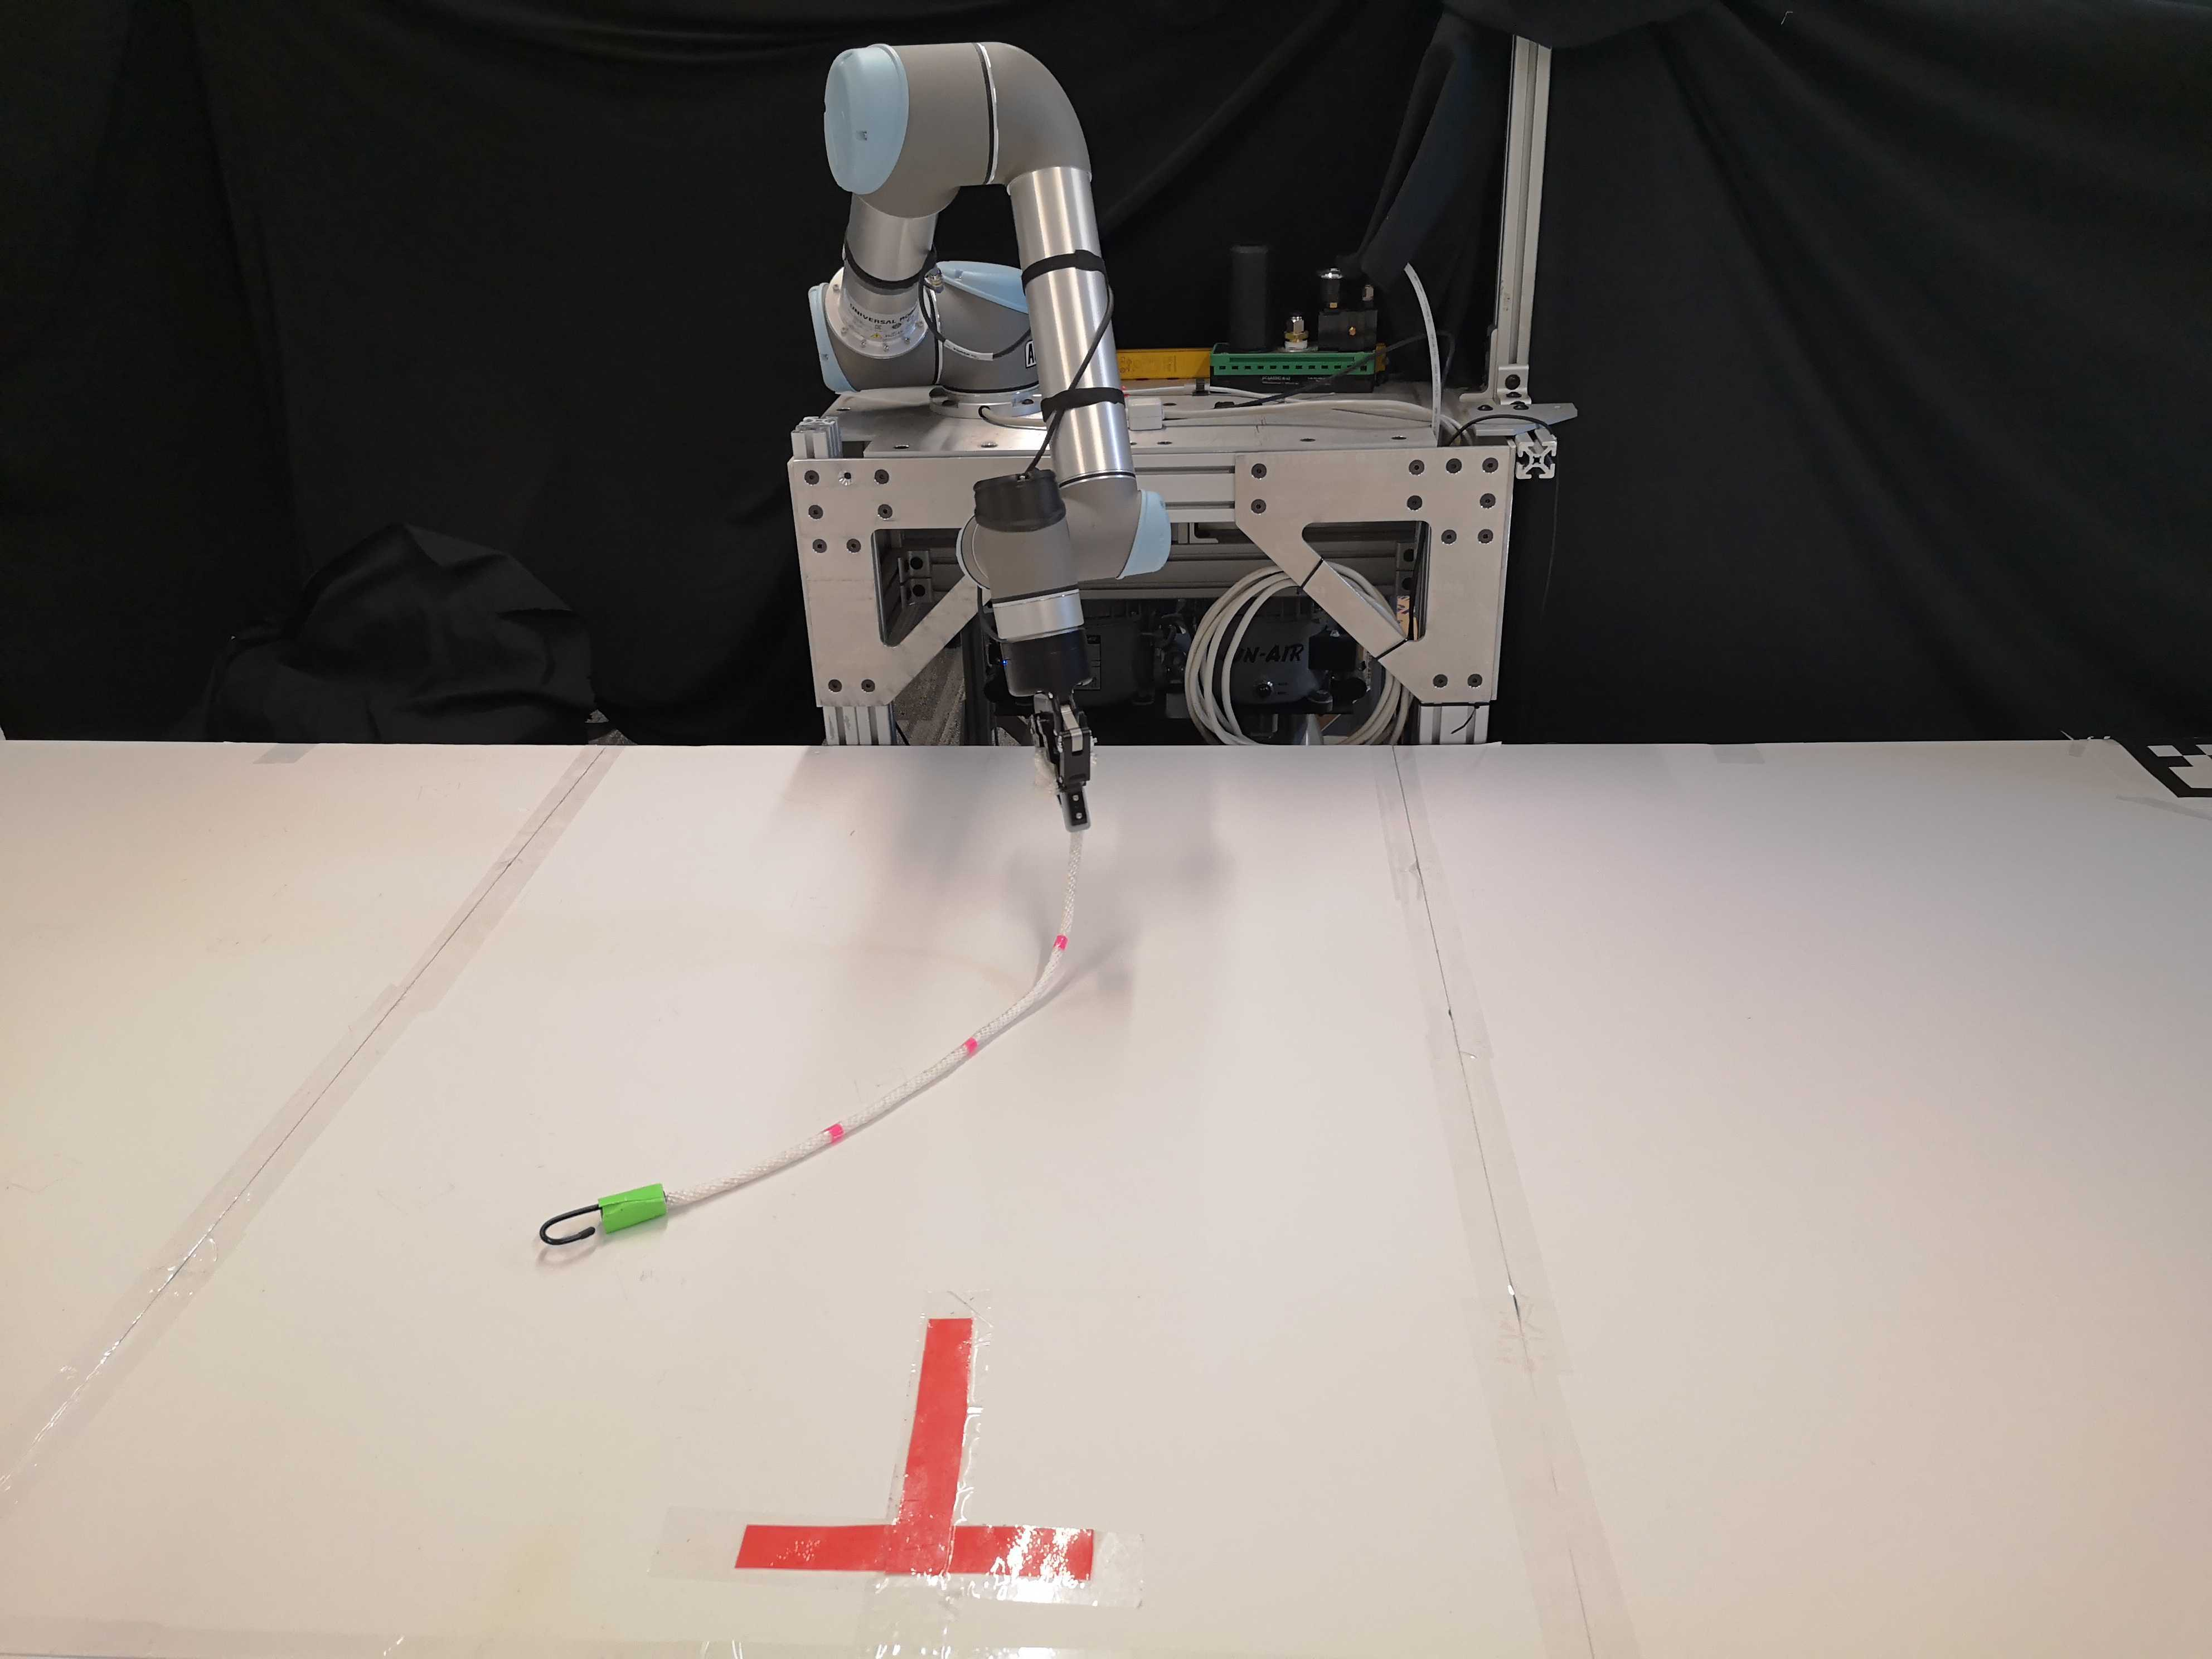
\includegraphics[width=0.24\textwidth]{ur5.jpg}}
%   \hfill
%    \subfloat[Side view]{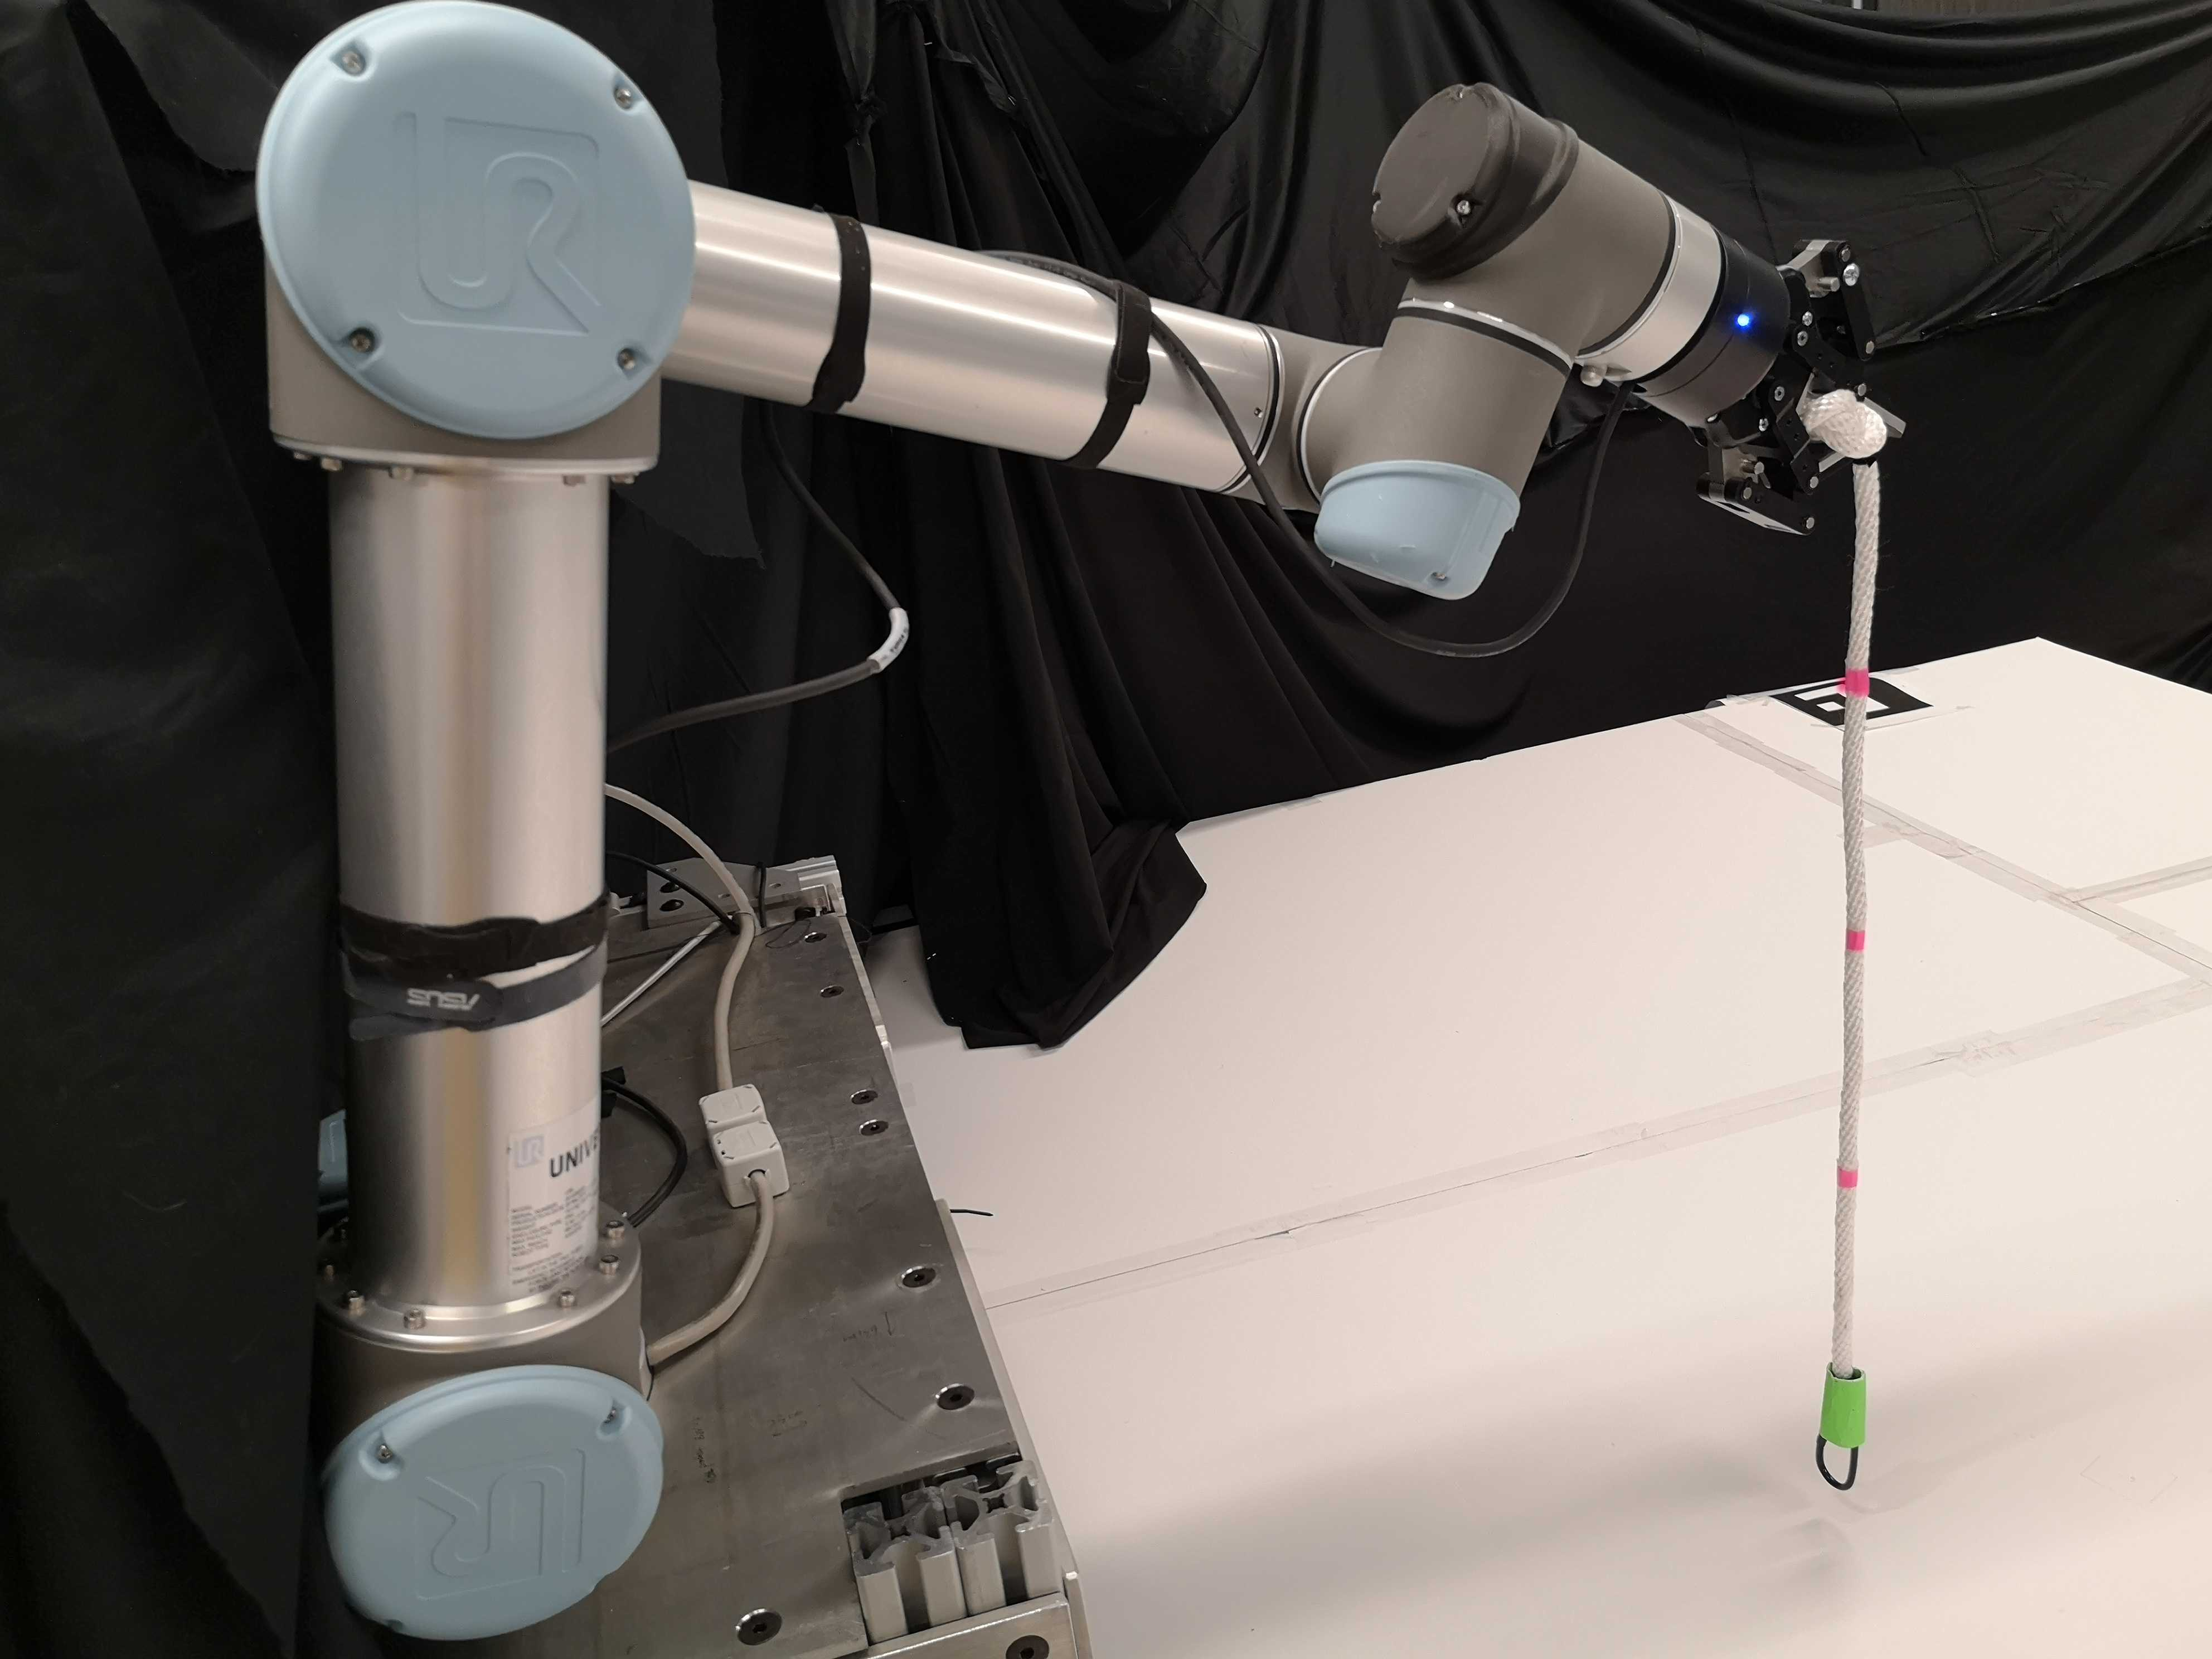
\includegraphics[width=0.24\textwidth]{ur5side.jpg}}
%   \caption{Physical experiment setup where the UR5 robot is holding a white cable with a green marker on the end to track the motion. The red T shaped markers are for image to real world coordinate transformation.\raven{will take better pictures} } 
%   \label{fig:ur5}
% \end{figure}


\subsection{Experiment Protocol}\label{ssection:protocol}

For each cable, we compare performance on 32 fixed target locations. \daniel{Will fix, Prof G asked this section to be modified in 3/1 feedback, we probably don't want to say targets are images since we really take a point in the image...} Each target location is extracted from an overhead image of the workspace with a green marker indicating the desired cable endpoint location. We sample the target locations symmetrically and to cover most of the workspace, as shown in Figure~\ref{fig:results-1}.
% We manually sample 15 target locations on the right side of the robot base and take the images. We then generate another 15 target locations by flipping the images horizontally such that we get 30 target locations in total that are symmetrical to the y axis of the robot base. We manually sample another 2 target locations in the center as a compliment. We use the same 32 target locations for all cables to consistently evaluate model performance. 

\subsubsection{System Parameter Selection}

\begin{figure}[t]
\center
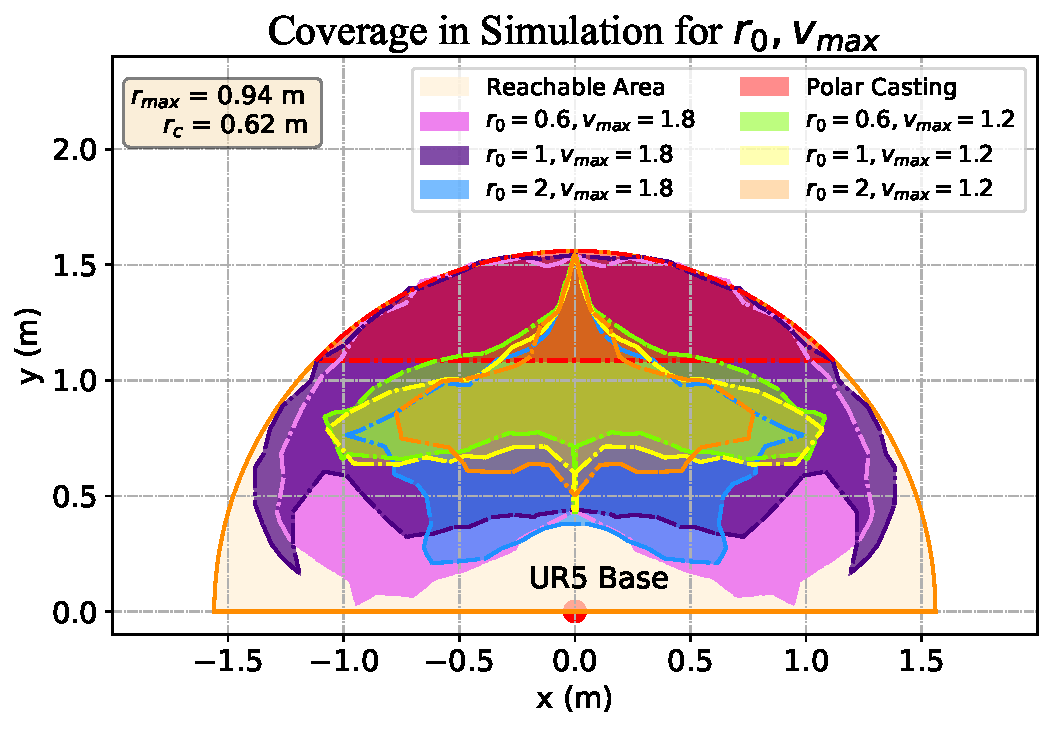
\includegraphics[width=0.49\textwidth]{figures/Coverage_Comparison.pdf}
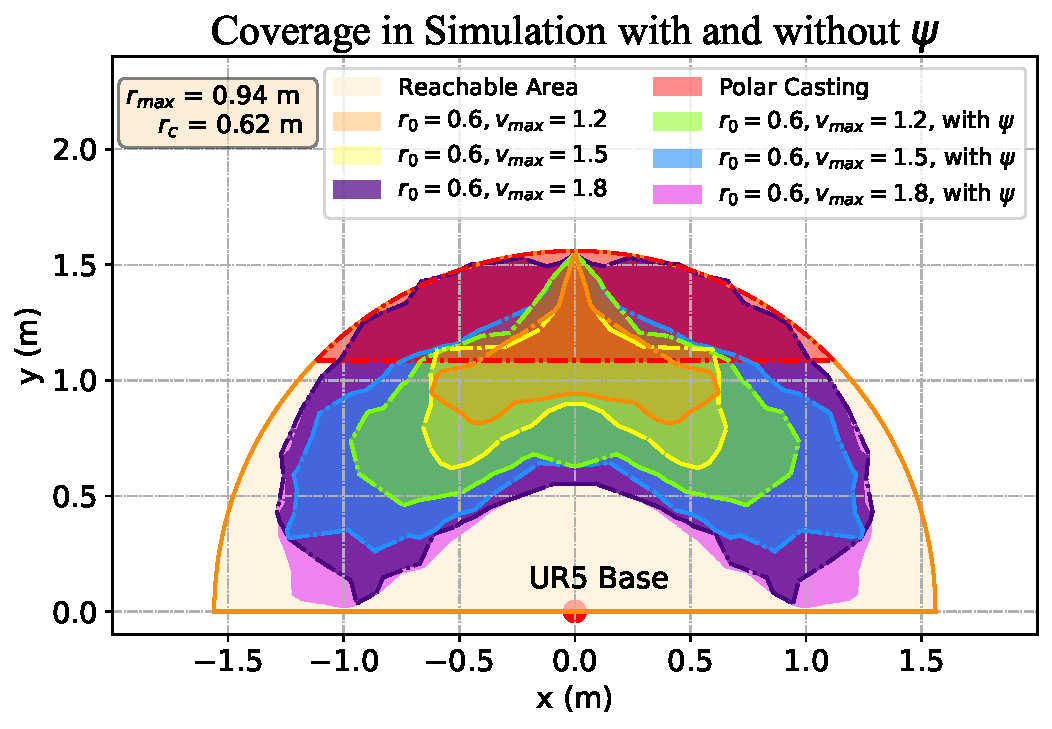
\includegraphics[width=0.49\textwidth]{figures/Coverage_Comparison_wrist.pdf}
\caption{
Plots showing the area on the workspace plane that is reachable by the cable endpoint across sampled trajectories for each system parameter combination in simulation, where parameters were tuned to match Cable 1. The reachable area for the cable endpoint is defined by a semicircle with radius $r_{\rm max} + r_c$. Each plot is generated by executing grid sampled actions $(\theta_1, \theta_2, r_2)$ with $\theta_1 < 0$ and $\theta_2 > 0$ in the simulator, reflecting endpoints across the vertical axis due to symmetrical actions, and applying a concave hull to the coordinates of the endpoints. All planar actions can achieve coverage beyond the area reachable by polar casting. \Vincent{We should justify why we reflect the points across the x axis}  \Lawrence{TODO: Modify the caption.}
}
\label{fig:coverage}
\end{figure}

To find the best $(r_0, \vmax)$ combination, we perform a grid search in simulation and real, with the goals of maximizing endpoint coverage and repeatability. We try $r_0 \in \{0.6,1,2\}$ and $\vmax \in \{1.2,1.8\}$ for $2\times3=6$ combinations. For each combination of $r_0$ and $\vmax$, we generate actions $\ba=(\theta_1,\theta_2,r_2)$ in via grid sampling, choosing the bounds for each parameter such that the trajectory does not violate any joint limits. We generate $15\times15\times15$ actions with $15$ values for each parameter and execute them in the simulator to evaluate the coverage of the end points.

% Then we generate $3\times3\times3$ actions and execute them in real to evaluate the coverage. 
Aggressive actions tends to give higher coverage, however generally bring more uncertainty resulting in less repeatability. We evaluate the \emph{repeatability} of the actions by repeating the \textbf{same} action given by the model five times in physical environment and calculate the variance of the distance between the end position of cable and the mean position.

We pick the combination of $r_0$ and $\vmax$ with maximizing coverage while maintaining repeatability as our final setting.

With the best $r_0$ combination, we further validate the importance of the additional wrist rotation parameter $\psi$ for $\vmax \in \{1.2,1.5,1.8\}$. We generate $15\times15\times15$ actions for $a=(\theta_1,\theta_2,r_2)$ and $10\times10\times10\times5$ actions for $a=(\theta_1,\theta_2,r_2, \psi)$ and execute them in real to evaluate the repeatability.
% Then we generate $3\times3\times3\times3$ actions and execute them in real to evaluate the coverage.

\subsubsection{Model Evaluation}
After selecting the most ideal system parameters $(r_0, \vmax)$ for coverage and repeatability, we use actions generated with these fixed values to learn a forward dynamics model as in Section~\ref{ssec:supervised}. To achieve the task of manipulating the cable such that the endpoint goes to the target position on the right side of the workspace, we sample 50,000 candidate actions using a grid sample on the joint-limit-abiding action parameters, and select the action that minimizes the $L^2$ distance between the predicted cable endpoint given by the learned dynamics model and desired cable endpoint. For target positions on the other side, we flip the target position to the right side and flip the action.
% We apply an HSV mask to isolate the green target marker in the pre-processed image observation and use contour detection to extract the pixel location of the target, which is then converted to corresponding $(x, y)$ coordinates in simulation. For our learning based method, we uniformly sample 1,000 actions such that $\ba$ produce trajectories that are within joint limit, and execute the action that minimizes the $\ell_2$ distance between the predicted cable endpoint from the dynamics model and desired cable endpoint.

Since some edge target positions require more stochastic actions to arrive, we evaluate the \emph{repeatability} of the target locations by repeating the \textbf{same} action output by the model three times and calculate the mean and variance of the distance between the end position of cable and the target position. The median and variance distance of each target position are reported.
% To evaluate the \emph{robustness} of the models, for each target position, we run the model three times to get three \textbf{different} actions. \Lawrence{There is no more robustness analysis now since all methods are deterministic. }
% The success rate for each target location is then defined as the number of successful actions out of three. A solution is considered to be successful if the distance between the endpoint of the cable and the target is lower than $20cm$.


\section{Results}\label{sec:results}

In this section, we report results for dynamic planar cable manipulation in simulation and real.

\subsection{System Comparison}
We compare the performance of models across various $(r_0, \vmax)$ values and perform an ablation study for including $\psi$ in the action (see Equation~\ref{eq:act2_wrist}).
\subsubsection{Coverage}
 From simulation, we find that $r_0 = 0.6, \vmax = 1.8$ provides the maximal coverage of $74\%$ of the reachable workspace, defined to be a semicircle with radius $r_{\rm max} + r_c$. Larger $r_0$ and smaller $\vmax$ result in a decrease in coverage. This is visualized in the top of Figure \ref{fig:coverage}. The bottom of Figure \ref{fig:coverage} compares the coverage with and without $\psi$ using $r_0 = 0.6$. From the graph, we can see that adding $\psi$ notably increases coverage, confirming our hypothesis in Section \ref{ssec:action}. Moreover, both $\vmax =1.5$ and $\vmax = 1.8$ provide sufficient coverage to reach targets on the workspace. The coverage map in simulation is shown in Figure.~\ref{fig:coverage}.
\subsubsection{Repeatability}
We observe that $\vmax = 1.2$ produces the most repeatable actions with an average standard deviation of \SI{8.9e-3}{\meter} compared to \SI{3.4e-1}{\meter} for $\vmax = 1.8$, but offers minimal coverage $22.3\%$.  Adding $\psi$ increases the standard deviation by 40\% - 115\%, but including $\vmax = 1.5$ with $\psi$ is still more repeatable than $\vmax=1.8$ without $\psi$. We thus choose $r_0 = 0.6$, $\vmax = 1.5$ to maximize coverage while maintaining repeatability, and include $\psi$ to increase coverage by $198\%$.

\begin{figure}[!tbp]
    \centering
    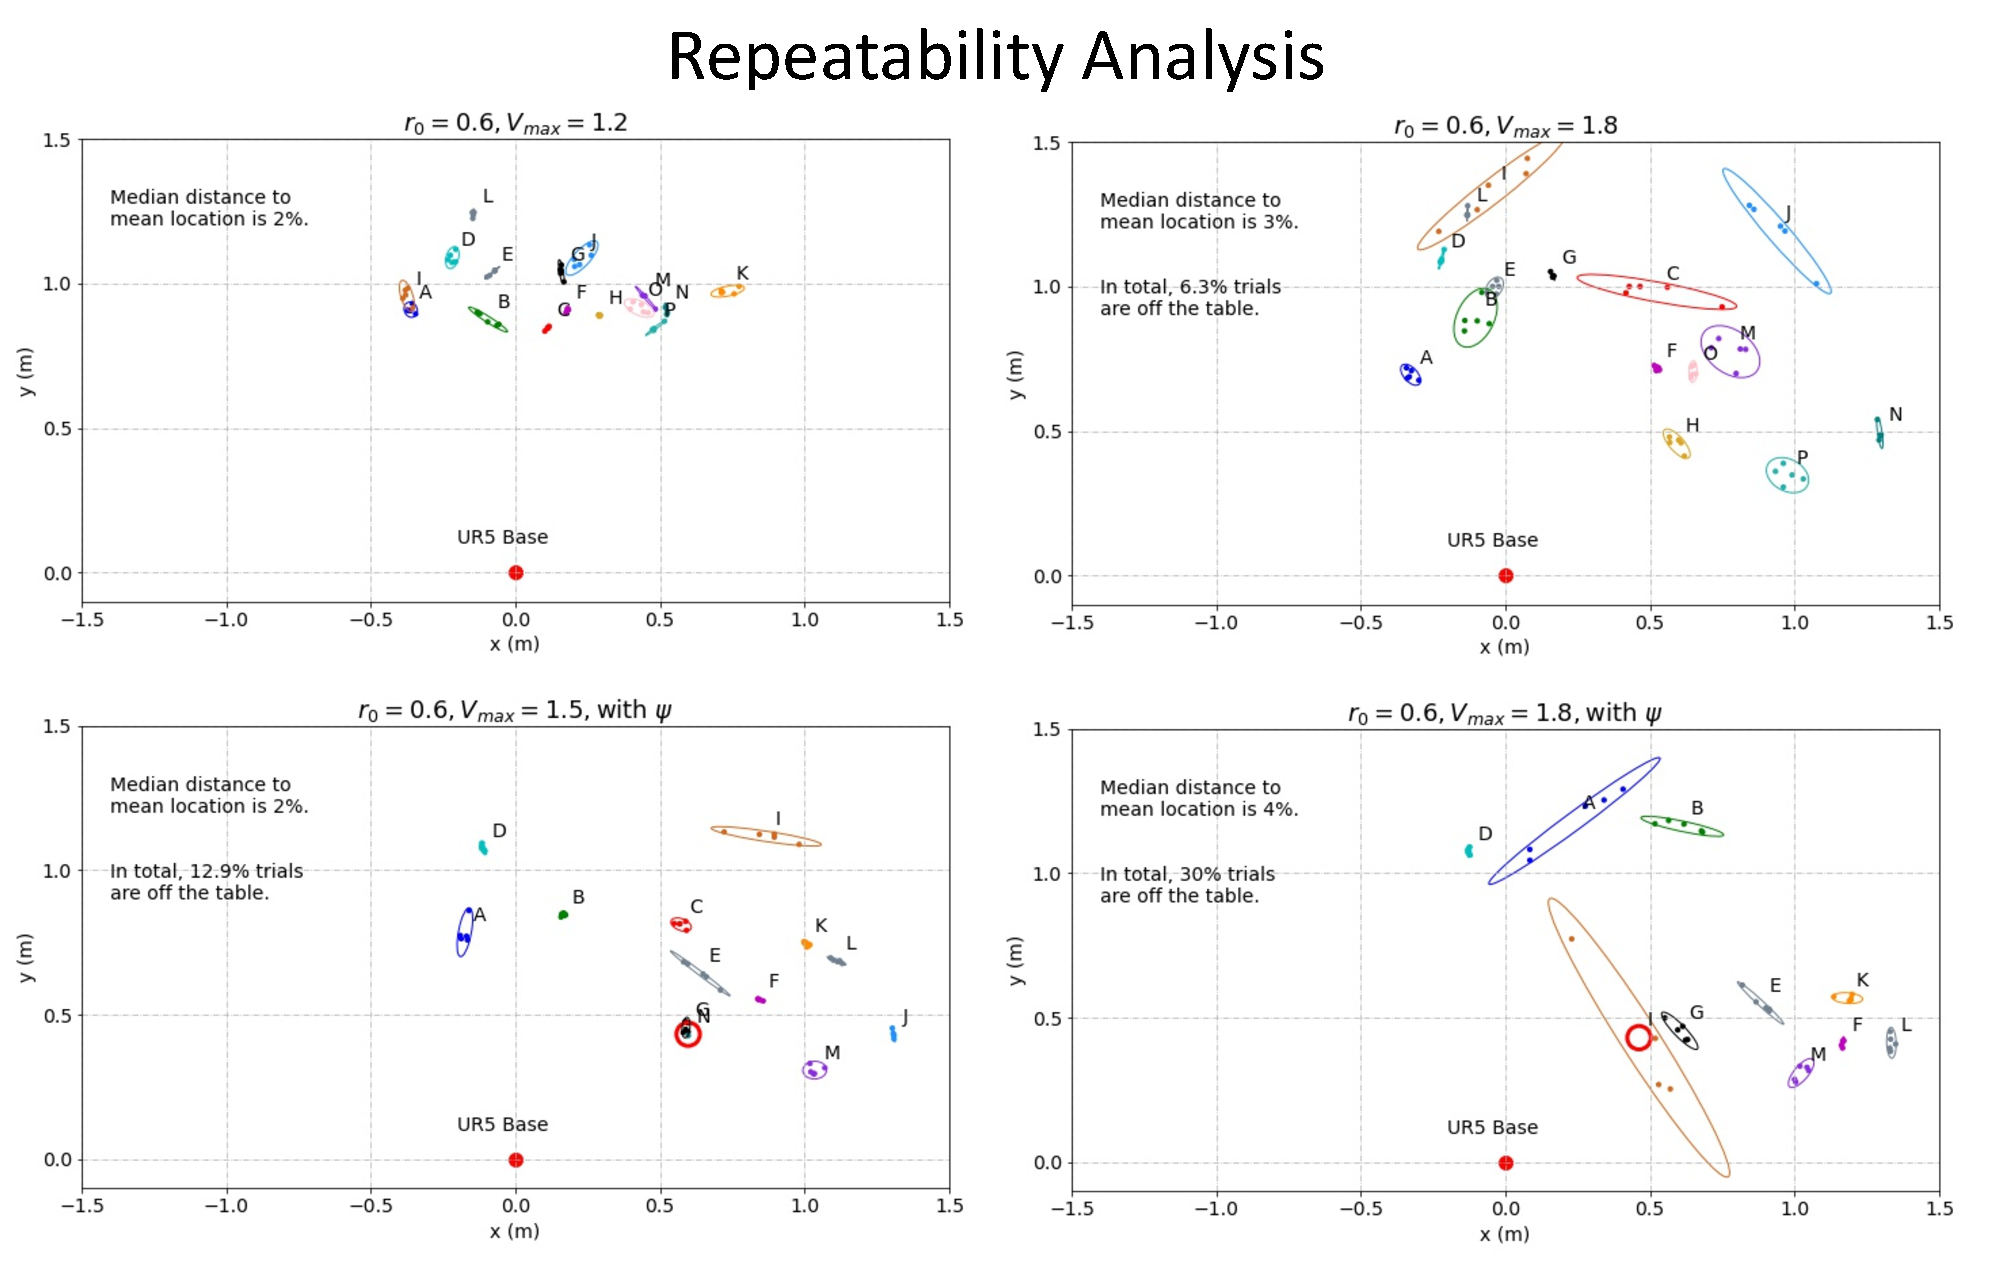
\includegraphics[width=\columnwidth]{figures/Repeatability_Analysis.pdf}
    \caption{
    Repeatability analysis for cable 1 where repeatability is represented by normalized Gaussian distributions. The position of each point represents the average endpoint location across 5 trials with the same action, and the color (i.e., intensity of the distribution) represents the standard deviation across the 5 trials, expressed in percentages of cable length (0.62~m).
}
\label{fig:repeat}
\end{figure}
% Model 1 has $r_0 = 0.2$ and action parameterization 1. Model 2 has $r_0 = 0.6$ and action parameterization 2. Model 3 has $r_0 = 0.6$ and action parameterization 1. We analyze the coverage of models generated in simulation as shown in Figure~\ref{fig:coverage}. The results show a wider coverage on side of model 3 brought by the addition trajectory parameter of wrist rotation angle $\psi$. A wider range in the center of model 1 aligns with the fact that smaller $r_0$ corresponds to more curvy splines that narrows the coverage on the side but extend the coverage in the center. The results of physical experiments on cable 1 for all the three models without any fine tuning are summarized in Table~\ref{tab:error} which emphasizes the importance of $\psi$. By comparing both the coverage and physical success rate, we use the setting of model 2 for subsequent experiments.

\begin{table}[ht!]
  \setlength\tabcolsep{5.0pt}
  %\vspace{-1em}
  \centering
  \caption{
    Physical evaluation results of the 2 baselines and $f_{\rm inv}$ on cable 1. All distances are in meters. \jonathan{Also show distances in units where 1 unit = radius of the reachable semicircle}
    \Lawrence{For relative error, are we using the cable length or cable length + robot arm length?} \jonathan{cable length + robot arm length}
  }
  \small
  \begin{tabular}{@{}lrrrrr}
  \toprule
  Model & Median & Std. & Min & Max & \% err. \\
  \midrule
Polar Casting & 0.267  & 0.217 & 0.024 & 0.700 & 17.1~\%  \\
Model GP & 0.180  & XXX & 0.035 & 0.979 & 11.5~\% \\
$f_{\rm inv}$ $\mathcal{D}_{\rm real}$ & 0.366  & 0.165 & 0.051 & 0.724 & 23.5~\% \\
$f_{\rm inv}$ $\mathcal{D}_{\rm sim}$ & XX  & XXX & XX& XX& XX~\% \\
$f_{\rm inv}$ $\mathcal{D}_{\rm sim} + \rm finetune$ & XX  & XX & XX & XX & XX~\% \\
  \toprule
  \end{tabular}
  %\vspace{-0.5em}
  \label{tab:error}
\end{table}  

\subsection{Physical Evaluation Results}
We evaluate 3 models on Cable 1, which are trained on only $\mathcal{D}_{\rm real}$, only $\mathcal{D}_{\rm sim}$, and $\mathcal{D}_{\rm sim}$ with fine-tuning on $\mathcal{D}_{\rm real}$. We find that training on $\mathcal{D}_{\rm sim}$ and fine-tuning on $\mathcal{D}_{\rm real}$ yields the best performance. We generate $\mathcal{D}_{\rm real}$ and $\mathcal{D}_{\rm sim}$ using system parameters $r_0=0.6, v_{max}=1.5$. The physical evaluation results for 32 targets are summarized in Table~\ref{tab:results}. We find that the best model produces actions that have a median distance of \SI{0.143}{\meter} from the target. Compared to the baselines, the inverse model has a lower median distance to the target. The GP model has a low median distance, but is highly inaccurate for certain target points with a maximum distance of \SI{0.979}{\meter}. Although polar casting is accurate for targets within its reachability,  the limited coverage greatly reduces its median distance. $f_{\rm inv}$ $\mathcal{D}_{\rm real}$ performs particularly poorly, most likely as a result of overfitting to the small size of $\mathcal{D}_{\rm real}$, supporting the need for $f_{\rm inv}$ $\mathcal{D}_{\rm sim}$. Fine-tuning on 200 real examples is also shown to improve accuracy. \jonathan{Include error heatmap}
\daniel{TODO adjust the numbers, we need FAR more analysis here, also qualitative results, failure cases (next subsection), etc.}

\begin{table}[ht!]
  \setlength\tabcolsep{5.0pt}
  %\vspace{-1em}
  \centering
  \caption{
    Physical evaluation results of 3 cables (see Figure~\ref{fig:cables}) with 32 target positions for each cable. The model used is $f_{\rm inv}$ $\mathcal{D}_{\rm sim} + \rm finetune$. Min and Max show the minimum and maximum distance between end point and targets among 32 targets. \jonathan{Distances are normalized by cable length} \Lawrence{The standard deviation I filled in is across targets, not between trials for each target.}
  }
  \small
  \begin{tabular}{@{}lrrrrr}
  \toprule
  Cable      & Median  & Std.  & Min & Max & \% err.  \\
  \midrule
  Cable 1    & 0.143 & 0.115 & 0.024 & 0.466 & XX  \\
  Cable 2    & 0.159 & 0.111 & 0.041 & 0.478 & XX  \\
  Cable 3   & 0.226 & 0.106 & 0.068 & 0.458 & XX \\
  \toprule
  \end{tabular}
  %\vspace{-0.5em}
  \label{tab:results}
\end{table}  

\begin{figure}[t]
\center
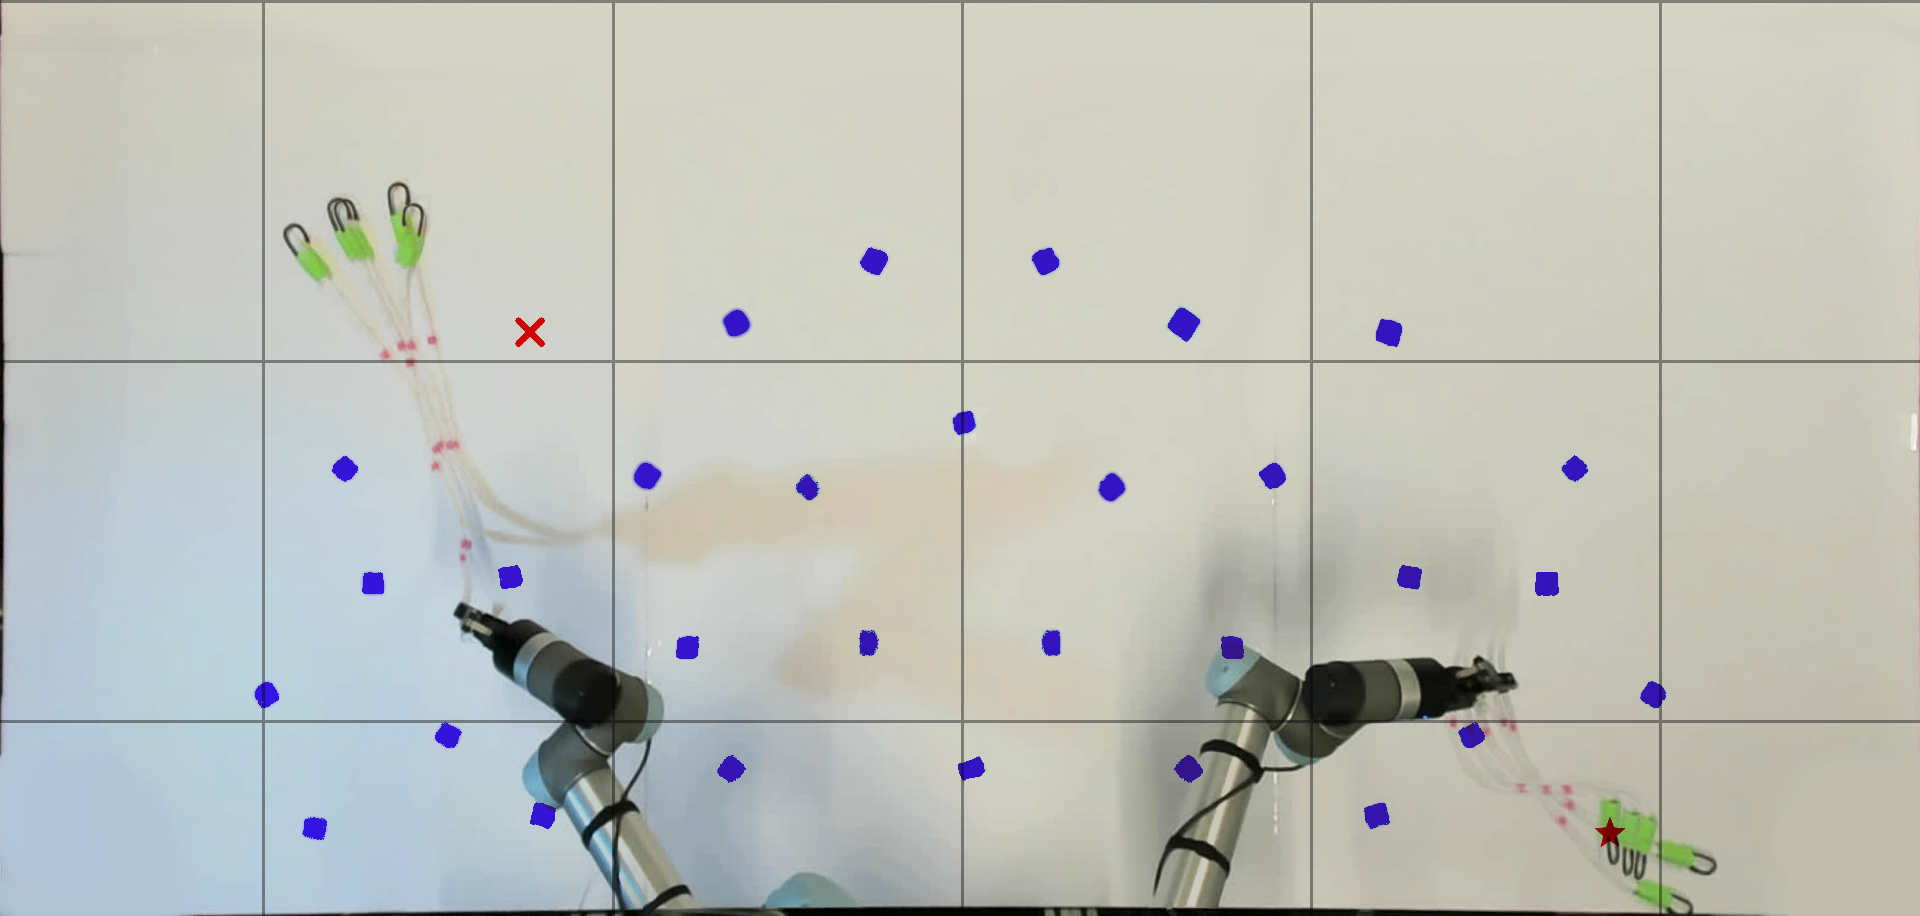
\includegraphics[width=0.49\textwidth]{figures/gridlines.png}
\caption{The 32 target positions on the workspace plane, shown with small tape. The target positions are chosen to cover most of the reachable space to thoroughly evaluate the model performance. The grid lines shown are 0.5 m apart. There are 5 trials of a successful case, marked by the star target, and 5 trials of a failure case, marked by the red cross. The successful case has median endpoint deviation of 0.05 m, while the unsuccessful case has a median endpoint deviation of 0.33 m.}
%\vspace*{-10pt}
\label{fig:results-1}
\end{figure}

\subsubsection{Repeatability}
We evaluate the repeatability for all 32 target positions for all cables, by repeating each output action 5 times per target. The results are shown in Figure~\ref{fig:repeat}. We can see points with higher standard deviation also have higher error implying those points are more difficult to reach. $f_{\rm inv}$ $\mathcal{D}_{\rm sim}$ has a lower standard deviation than the baselines and  $f_{\rm inv}$ $\mathcal{D}_{\rm real}$, suggesting the model is able to learn and favor motions that are more reliably able to reach the target. $f_{\rm inv}$ $\mathcal{D}_{\rm sim} + \rm finetune$ can achieves consistent repeatability across the 3 cables.

% \begin{figure}[!tbp]
%   %\begin{minipage}[b]{0.40\textwidth}
%         \includegraphics[width=\columnwidth]{figures/targets_with_gridlines.png}
%     \caption{
%     The 32 target positions on the workspace plane, shown with small tape. The target positions are chosen to cover most of the reachable space to thoroughly evaluate the model performance. \daniel{Need to: (1) add a scale to indicate true length, (2) better align with figure below} % \Lawrence{(1) still needs to be done.} \jeffi{Can we overlay a grid to match the fig.~\ref{fig:repeat}?}
%     }
%     \label{fig:target}
%   %\end{minipage}
% \end{figure}

\begin{figure}[!tbp]
    \centering
    \includegraphics[width=0.45\columnwidth]{figures/Error_Heatmap_s2r_model_cable1_0304_notfinetuned_imgs.jpg}
    \includegraphics[width=0.45\columnwidth]{figures/Error_Heatmap_s2r_model_cable1_0304_finetuned_imgs.jpg}
    \includegraphics[width=0.45\columnwidth]{figures/Error_Heatmap_s2r_model_cable2_0304_notfinetuned_imgs.jpg}
    \includegraphics[width=0.45\columnwidth]{figures/Error_Heatmap_s2r_model_cable2_0304_finetuned_imgs.jpg}
    \includegraphics[width=0.45\columnwidth]{figures/Error_Heatmap_s2r_model_cable3_0304_notfinetuned_imgs.jpg}
    \includegraphics[width=0.45\columnwidth]{figures/Error_Heatmap_s2r_model_cable3_0304_finetuned_imgs.jpg}
    \caption{
    Repeatability analysis for cable 1 where repeatability is represented by normalized Gaussian distributions. The position of each point represents the average endpoint location across 5 trials with the same action, and the color (i.e., intensity of the distribution) represents the standard deviation across the 5 trials, expressed in percentages of cable length (0.62~m).
}
\label{fig:repeat_multi_cable}
\end{figure}
\subsubsection{Error Analysis} Certain targets can be consistently reached with lower distances to target than others, as seen in Figure \ref{fig:repeat_multi_cable} \Lawrence{The figures are WIP}. We attribute the error to two errors, learning error and sim-to-real error. Evaluating $f_{\rm inv}$ $\mathcal{D}_{\rm sim}$ on the same 32 targets in simulation achieves a median distance of \SI{0.054}{\meter}, which represents the difficulty of learning the forward dynamics of a complex cable via a neural network. The sim-to-real error is demonstrated by Table \ref{tab:tuning}, however, while the sim-to-real gap was least prevalent for Cable 3, it is surprising that Cable 3 actually has the lowest performance. We conjecture that the cylindrical shape of the endpoint mass contributes to increased stochasticity and is thus more difficult to model, leading to a higher median distance than the other two cables. \jonathan{Describe qualitative examples of failure cases} While we modeled the extra mass at the endpoint, we may consider modeling irregular shapes to decrease the sim-to-real gap. \Lawrence{Not sure if we should put in another error heatmap or just use words to describe.}


% \daniel{WIP}. See Figure~\ref{fig:results-1}.

\section{Conclusion and Future Work}\label{sec:conclusion}

\daniel{Need to give better conclusion overview}

Experimental results suggest that a data-driven approach via simulator tuning is a promising for learning dynamic planar cable manipulation. The self-supervised data collection in a combination of simulated and real-world environments provides a procedure for efficiently adapting to cables with different properties.

When tuning the simulation parameters, we choose our optimization metric to be the 2D Euclidean distance from the simulated free end to the ground truth endpoint location at discrete time steps, assuming that endpoint location is sufficient to find parameters that model the cable. In future work, we plan to relax this assumption and explore additional ways to better tune the simulator.

The fine-tuning process relies on executing hundreds of trajectories in the physical setup, which may be infeasible in many other dynamic manipulation domains. Recently, dynamics randomization~\cite{dynamics_randomization_2018} has shown to aid in effectively transfer polices to real. Pre-training the learned model with trajectories executed with random dynamics could provide better initialization for transfer than a model trained on only a single set of parameters. Previous dynamics randomization literature has found that recurrent polices transfer more effectively with dynamics randomization than memoryless feedforward neural networks. However, as the current action parameterization is output in a single step, a recurrent network may not be applicable. 

We also note that this method relies on learning a separate set of simulation parameters and forward dynamics model for each cable. Another approach we will consider is a meta-learning approach such as MAML~\cite{maml}, which may assist with rapid adaptation to other cables to avoid learning parameters for each cable. 


% Daniel: don't make this tiny font.
\section*{Acknowledgments}

{\small 
This research was performed at the AUTOLAB at UC Berkeley in affiliation with the Berkeley AI Research (BAIR) Lab, the CITRIS ``People and Robots'' (CPAR) Initiative, and the Real-Time Intelligent Secure Execution (RISE) Lab. The authors were supported in part by donations from Toyota Research Institute and by equipment grants from PhotoNeo, NVidia, and Intuitive Surgical. Daniel Seita is supported by a Graduate Fellowship for STEM Diversity (GFSD). We thank our colleagues who provided helpful feedback, in particular Ashwin Balakrishna, Ellen Novoseller, and Brijen Thananjeyan.
}



% \clearpage Daniel: can do this if needed
\bibliographystyle{IEEEtranS}
\bibliography{example}
% Back to normal size.
\normalsize
\cleardoublepage
\appendices

%%%%%%%%%%%%
% APPENDIX %
%%%%%%%%%%%%

This appendix is structured as follows:

\begin{itemize}
    \item In Appendix~\ref{app:method-details} we discuss the proposed method in further detail.
    \item In Appendix~\ref{app:exp-details} we present experiment details.
    \item In Appendix~\ref{app:exp-results} we describe additional results.
\end{itemize}


\section{Additional Method Details}\label{app:method-details}

Here we describe additional details of the method.
\daniel{Maybe describe things like how we tuned things, etc. Could also describe how errors propagate throughout time as in Figure~\ref{fig:fly-fishing} but adapted to our setting.}

\subsection{Simulator Tuning via Differential Evolution}

\begin{table}[t]
  \setlength\tabcolsep{3.0pt}
  %\vspace{-1em}
  \centering
  \caption{
  PyBullet simulation parameters for dynamic cable manipulation tasks across all cables we test in physical experiments (see Figure~\ref{fig:cables}). The stiffness, friction, and damping constants are unit-less, and the mass per segment is in kilograms. \jeffi{We should minimally move this to the experiments section.  We may also consider moving the table to supplemental material. While its important for our experiments, it doesn't tell the reader much, other than the cables have different parameters.}
  } 
  \small
  \begin{tabular}{@{}lcccc}
  \toprule
  PyBullet       & & & & Range \\ 
  Hyperparameter & Cable 1 & Cable 2 & Cable 3  & Explored \\
  \midrule
  Twist stiffness       & 1.90 & 2.83 & 3.20 & $[0, 5]$ \\
  Bend stiffness        & 3.32 & 2.69 & 1.75 & $[0, 5]$ \\
  Mass per segment      & 1.66 & 1.93 & 0.60 & $[0.3, 2]$ \\
  Lateral friction      & 0.41 & 0.83 & 0.70 & $[0.3, 2]$ \\
  Spinning friction     & 0.01 & 0.01 & 0.04 & $[0, 0.1]$ \\
  Rolling friction      & 0.88 & 1.04 & 1.15 & $[0, 1.5]$ \\
  Scaled endpoint mass  & 4.34 & 4.28 & 3.52 & $[1\textrm{x}, 5\textrm{x}]$ \\
  Linear damping        & 0.62 & 0.83 & 0.45 & $[0, 1.5]$ \\
  Angular damping       & 12.2 & 8.74 & 1.10 & $[1, 20]$ \\
  Table friction        & 0.53 & 0.14 & 0.46 & $[0,1]$ \\
  \bottomrule
  \end{tabular}
  %\vspace{-0.5em}
  \label{tab:hparams-sim}
\end{table}

\daniel{Starting now, rest of paragraph, move to appendix}
\jeffi{I agree, and I would also like to see a summary of how DE works here, and an overview of our implementation.}
We use a ``best1bin'' strategy to optimize for the minimum deviation in trajectory across 80 different trajectories. In this technique, each child parameter array is created by either choosing a parameter for its parent array, or a combination of the current best (lowest cost) array and two random parameter arrays, where ${\rm Unif}(0, 1) > CR$ selects the parameter from the parent array. $CR$, the crossover probability, affects the frequency at which a child inherits a parameter from its parent, or from a mutated version of the most fit individual. An additional parameter, $F = {\rm Unif}(F_{\rm min}, F_{\rm max})$, is the differential weight. For each generation, $f \sim F$ is sampled, and a large $f$ increases the search space of the algorithm, but decreases convergence rate. We choose DE parameters that were consistent with Collins~et~al., because their results showed that DE was able to find PyBullet parameters that were more optimal than its default settings, in relatively low convergence time. We use $CR = 0.7$, $F = 0.5 - 1.0$, and population size of $N = 1D$, where $D$ is the number of simulation dynamics parameters. Convergence is set to be the standard deviation of the population reaching below $1\%$ of the population mean.

\begin{figure}[h]
\center
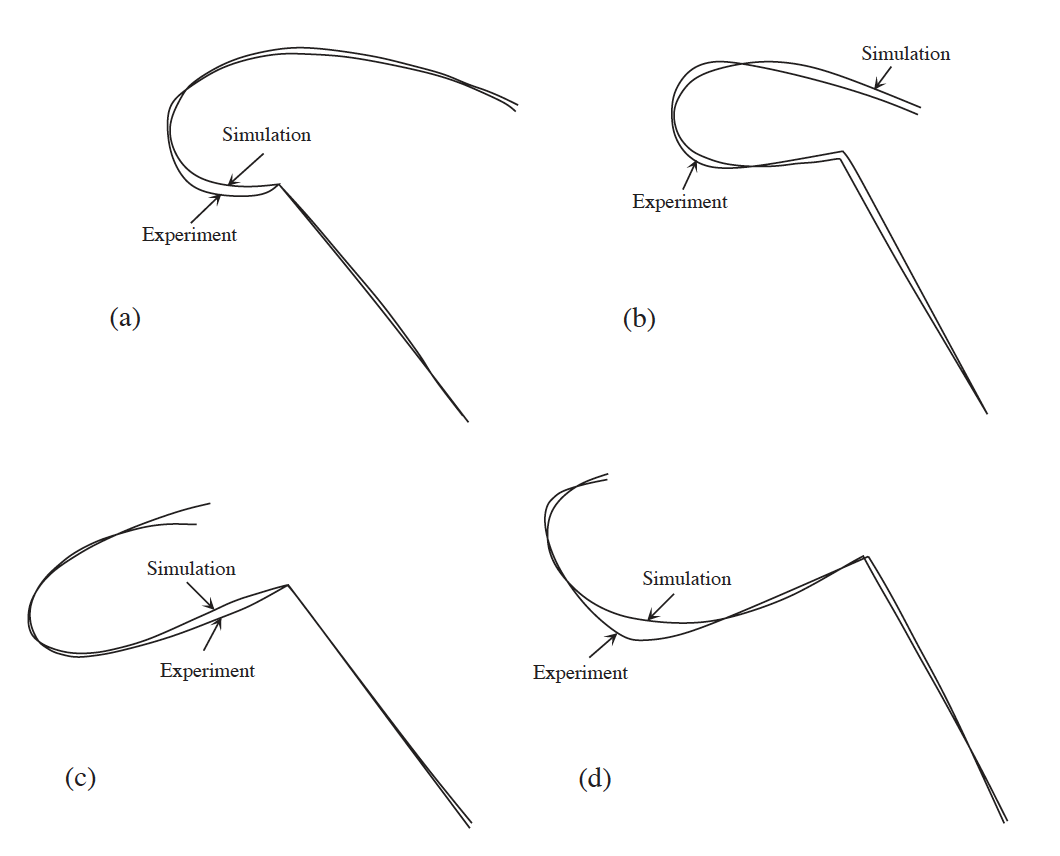
\includegraphics[width=0.3\textwidth]{real_vs_sim.png}
\caption{
\Lawrence{Maybe we can compare real vs sim as in the fly fishing paper? It would be nice to illustrate how the errors propagate through time} \daniel{Why is this figure here?} \Lawrence{I was thinking that it may be good to show the readers how our parameter tuning did by illustrating the sim to real gap visually. But we probably don't have time to do this anyway.} \daniel{Moving to appendix, I think something like this could be useful for further investigation}
}
\vspace*{-10pt}
\label{fig:fly-fishing}
\end{figure}

\begin{figure}[t]
\center
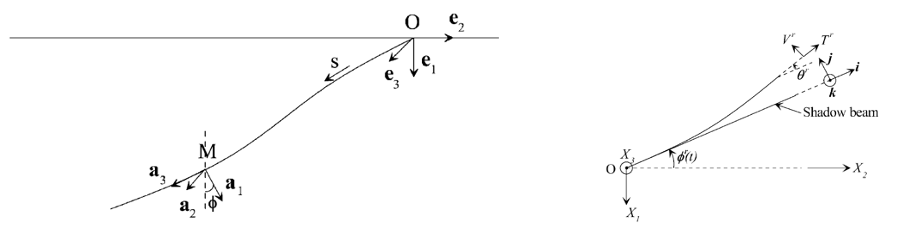
\includegraphics[width=0.49\textwidth]{param_illustration.png}
\caption{
\Lawrence{Maybe somewhere we can illustrate our action parameters as in the fly fishing paper?} \daniel{Why do we have this figure here?}\Lawrence{I am talking about the figure that Jonathan mentioned TODO. Just a placeholder, ours can be different.} \daniel{OK sounds good, let's iterate upon this figure}
}
\vspace*{-10pt}
\label{fig:action_param}
\end{figure}

\section{Additional Experiment Details}\label{app:exp-details}

Since the overhead camera is not perfectly parallel to the plane of the table, we put four fiducial markers on the corners of the foam boards. We process the image by using the fiducial markers to detect the corners of the table, crop out the residual area, and apply a perspective shift to mitigate perspective effects. 

Due to the irregular shapes of the hooks, we find that the end of the cable would bounce out in random directions when colliding with the table during the reset tossing motion. To mitigate this uncertainty, we pull the cable back slightly after the tossing motion to straighten the cable. In addition, the foam boards on the table can help in uncertainty reduction. 

\section{Additional Results}\label{app:exp-results}

\begin{figure*}[t]
\center
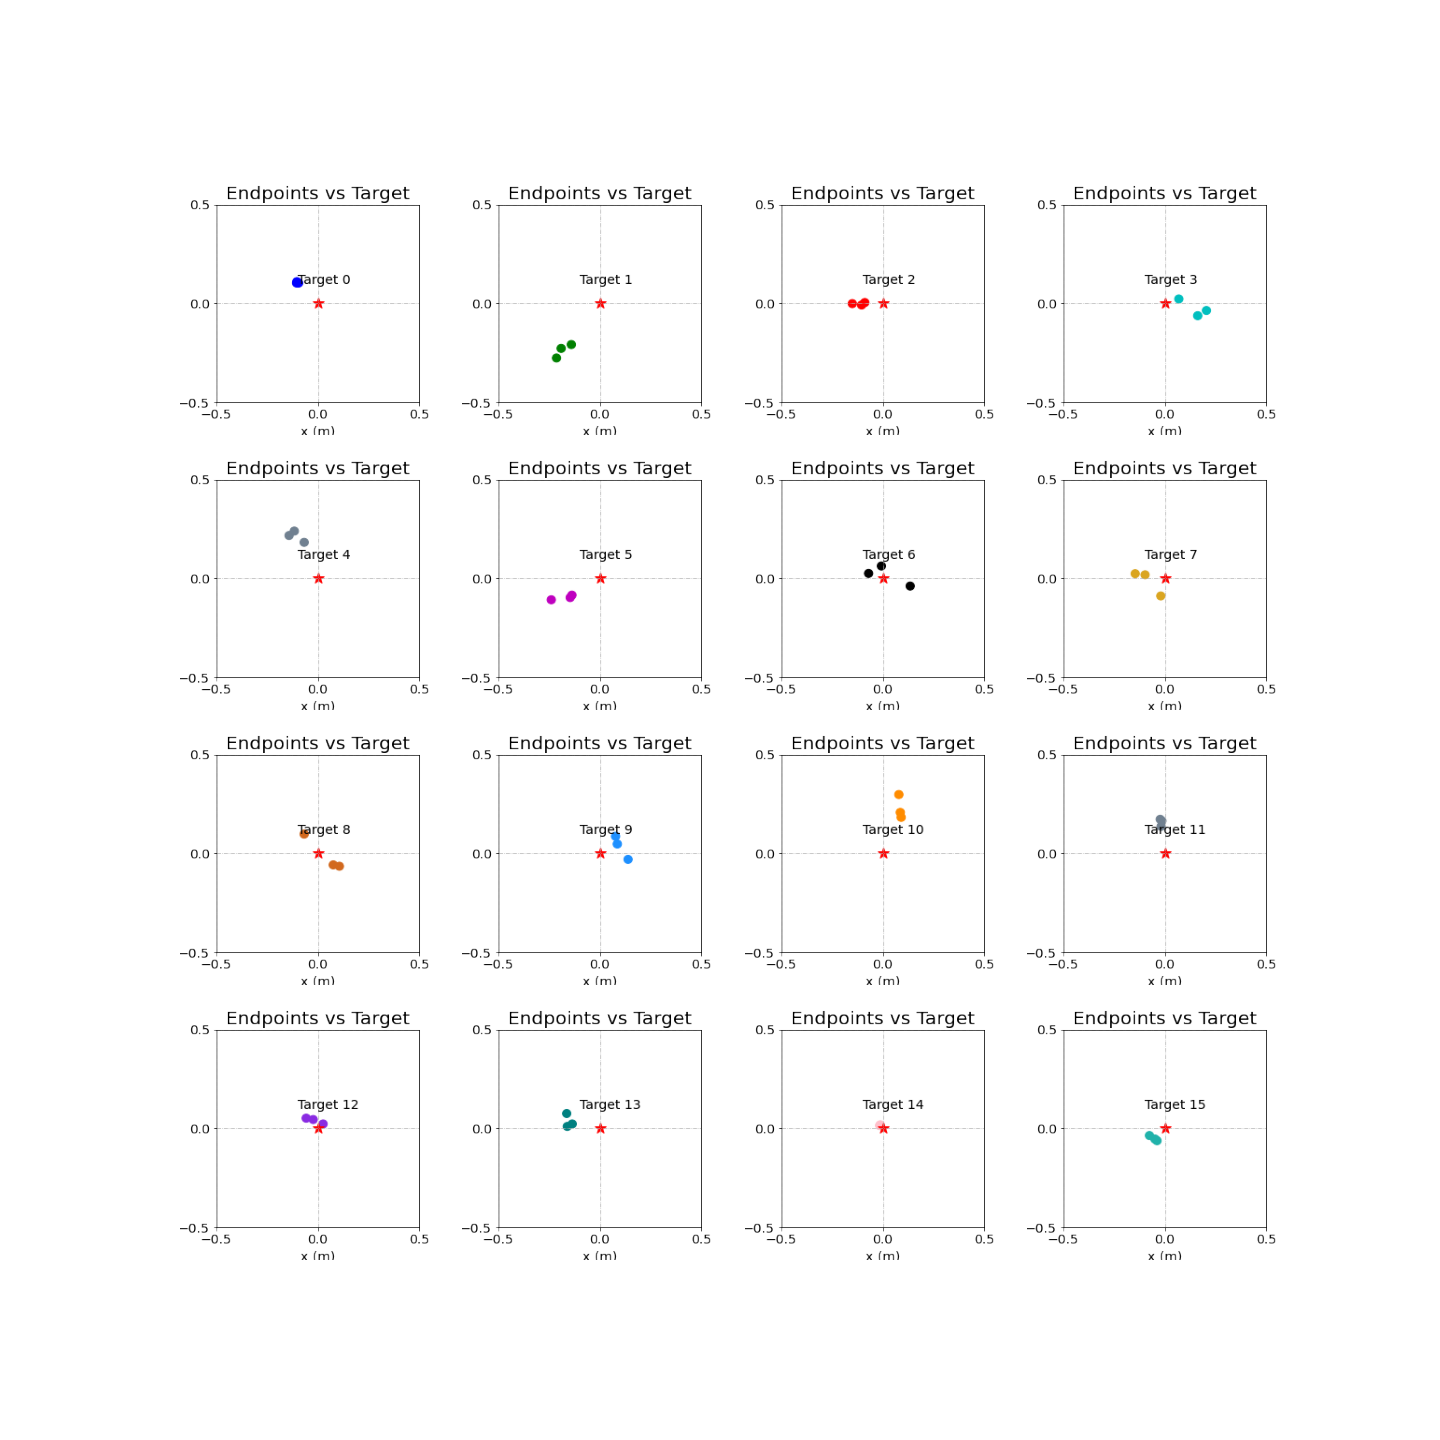
\includegraphics[width=0.98\textwidth]{combined.png}
\caption{
\daniel{Add caption, remove excess whitespace (are we using tight layout?)}
\Lawrence{Are we going to put this image in the appendix? If so, I will re-create the image with appropriate data. This is just half of the result as we have symmetric targets as well.} \jonathan{This is a temporary placeholder figure. We will update this when we obtain results for our most recent models}
}
%\vspace*{-10pt}
\label{fig:endpoints-1}
\end{figure*}

See Figure~\ref{fig:endpoints-1}? \daniel{Please describe}

  
\end{document}
